\documentclass[11pt]{article}
\usepackage[margin=1in]{geometry}
\usepackage{booktabs}
\usepackage{graphicx}
\usepackage{natbib}
\usepackage{amsmath}
\usepackage[hidelinks]{hyperref}
\graphicspath{{./}}

\title{Elective surgical allocation in Brazil's public health system: a statewide
benchmark from Goi\'as, 2019--2025}
\author{Gustavo Lombello Bargieri}
\date{November 2026}

\begin{document}
\maketitle

\begin{abstract}
\noindent
SUS-financed elective surgery in the Brazilian state of Goi\'as roughly doubled between 2019 and 2025.
Using all 2.72 million SUS hospital authorisations processed in the state (430,802 elective surgical admissions, 201 facilities), we describe the expansion and compare the observed geographic allocation with a capacitated assignment benchmark.
Facility-procedure activity in the record is intermittent: of 284 pairs observed in 2023 and not in 2019, 195 also recorded activity in 2020 to 2022 and account for 94 per cent of the group's cases, so an endpoint-year comparison classifies as new many pairs that appear in the intervening records.
Holding each pair to its peak three-month volume and scoring travel on a baseline 0--3 regional scale, the benchmark's mean cost score is 28.8, 30.6 and 29.1 per cent below the observed allocation's in 2019, 2023 and 2025 (0.595 vs 0.835, 0.587 vs 0.846, 0.642 vs 0.906), with no statistically detectable change between years.
These percentages describe the coded objective, not distance, and are conditional on construction: the sensitivity range across cost codings, zones, bed definitions, windows and noise-deflated caps is 23 to 55 per cent, and caps at annual mean volume give 6.2, 22.7 and 29.6 per cent with 0.3, 7.3 and 9.8 per cent of demand unassigned.
Utilisation of the constructed bed-day budget at the reported optimum is 0.13 to 0.21; one, three and six facilities use more than 95 per cent of it.
The benchmark is a diagnostic counterfactual, not an estimate of the system's production frontier, and Goi\'as residents treated in the Federal District are absent from the data.
\end{abstract}


\section{Introduction}
\label{sec:intro}

Between 2019 and 2025 the Brazilian state of Goi\'as roughly doubled its monthly
volume of elective surgery in the public health system, from 3{,}896 admissions
per month to 8{,}013, while urgent surgical volume rose by 15 per cent. The
increase is not pandemic recovery: elective volume had returned to its
pre-2020 level by early 2022 and stopped there, and the post-2022 level has no
precedent in the panel. This paper describes what that expansion consisted of and how far the resulting allocation sits from a transparent benchmark.

The paper asks four descriptive questions. Which facility-procedure pairs
account for the gain between 2019 and 2023, and do they appear in the intervening records? Were hospital beds limiting? How far is the realised allocation from the optimum of a
linear program that sends each municipality's patients to the facilities at least travel cost, and did the mean coded cost index change? And how much of what we compute
about the program's constraints survives our own tests? None of these questions identifies the cause of the expansion, and the paper does not.

We formulate the allocation of elective surgery across facilities as a
capacitated assignment problem with a travel-penalised access objective, and
solve it on administrative microdata covering 2{,}719{,}254 hospital
authorisation records, of which 430{,}802 are elective surgical admissions
across 201 facilities over 84 months. Four findings follow, each stated with the tests that bound it.

First, facility-procedure activity in the administrative record is intermittent, so a comparison of two endpoint years classifies as new many pairs that appear in the intervening records. A pair counts as active in a month when it records at least one elective surgical admission. Of the 284 pairs present in 2023 and absent in 2019,
carrying 27.5 per cent of 2023 elective volume, 195 are active in some month of 2020 to 2022 (median five active months and ten cases) and carry 94.2 per cent of the cases, so 25.9 of the 27.5 points are
pairs with earlier activity in the record, and 1.6 points are pairs with none; across the panel 1{,}028 of 1{,}179 pairs record at least one interruption of three consecutive months. This describes the record, not why a pair was dark in a given year. Of the 284 pairs' volume, 52 per cent is at facilities absent from SIH altogether, or 84 per cent on the broader test of absence from its elective subset.
Under the model's 2019-pair configuration and feasibility rules, 11.5 per cent of 2023 demand remains unassigned; with the 2023 pairs all of it is assigned. We make no attribution of the change between
pairs and capacity (Table~\ref{tab:decomp}).

Second, the constructed bed-day budget was slack in aggregate, and a few facilities used nearly all of it. The budget is SUS surgical beds times 30 days, net of urgent surgical bed-days, and is not a measure of staffed beds. Aggregate utilisation of net surgical bed-days at the reported optimum is 0.132 in 2019,
0.178 in 2023 and 0.215 in 2025 (0.06 to 0.09 when every admission is netted against all inpatient beds), and one, three and six of 131, 131 and 145 facilities use
more than 95 per cent of their bed-day budget. Dropping the bed row raises the benchmark gap by 0.0, 3.5 and 2.4 points, because 1, 3 and 5 facilities would then exceed their budget.
Beds are counted at full occupancy; operating-room sessions, surgeons and anaesthetists are not modelled.

Third, a transparent benchmark shows no detectable change in the gap, and its level depends on construction. Under the peak-volume cap and the baseline 0--3 regional cost score, the optimum's mean cost index is 28.8, 30.6 and 29.1 per cent lower than the observed
allocation's (0.595, 0.587 and 0.642 against 0.835, 0.846 and 0.906) (the gap is (observed $-$ optimum) / observed; 29 per cent lower corresponds to the observed index being about 41 per cent above the optimum). The score is 0 to 3 by the regional boundary crossed, and the program sums it, so it assumes equal steps between categories; the gap describes the coded objective, not kilometres or journey time, and alternative codings are in Table~\ref{tab:measure}. Differences between years are not distinguishable from zero, with
intervals about nine points wide, so this is no detectable change and not evidence of equality. The level ranges from 23 to 55 per cent across cost codings, origin zone systems (including the official health regions), bed definitions, estimation windows
and caps deflated for counting noise, and is 6 per cent in 2019 when each pair is held to its annual mean volume, with 0.3 per cent of demand then unserved (Table~\ref{tab:measure}). The observed mean index did not fall: it rose from 0.835 to 0.846 to 0.906.

Fourth, what we can say about the constraints is limited. The cap is a peak, not a demonstrated ceiling. The number of facilities at their cap is not identified (in 2023 a proved minimum of 44 of 131 and a largest value found of 107 across optima of equal cost);
disjointness of bed-bound and cap-bound facilities is a property of the reported optimum, and an overlap is attainable at other optima in 2019 and 2025; the cap test is a low-power non-rejection; and the explanation ``flatter monthly series'' for the fall in aggregate cap over demand is not supported (Section~\ref{sec:capnull}).
Goi\'as residents treated in the Federal District are missing from the data, so we draw no conclusion about the Entorno. An exploratory extension that lets the program open new pairs is in Appendix~\ref{app:explore}. Taken together, the benchmark is a diagnostic counterfactual under a historical-volume feasibility rule: it says how far the observed allocation sits from what that rule permits, not what the system could produce.

The implication for modelling is limited. A scheduling model that takes the machine set as given cannot represent a change in which
facility-procedure pairs exist, and would attribute to allocation a gain that came with pairs and their caps. The
fixed-machine-set assumption, usually a modelling convenience, is here a substantive question, which this paper treats descriptively.

Two features of the setting make the model's capacity constraint non-obvious and
are established empirically before it is imposed. Capacity is consumed in
bed-days rather than cases. Across elective admissions in calendar 2023, mean
length of stay is 1.57 days at facilities under municipal contract
administration and 2.32 days at state-administered ones, a ratio of 1.48. Case
mix explains none of it --- both directions of reweighting at ten-digit
procedure detail bracket the raw gap --- and complexity runs the wrong way,
since municipal-administered facilities perform proportionally more
high-complexity work, not less. A case is therefore not a fixed claim on
capacity, and a model that rations cases rather than bed-days would misprice
every facility whose stays are short. And the capacity that exists is unequally
free: total bed occupancy over 2023--25 is 0.33 at municipal-administered
facilities against 0.79 at state-administered ones, so
total bed occupancy is lower at municipal-administered facilities, indicating more bed slack by this measure; the data do not establish the marginal operational cost of an additional elective case.

The paper contributes in three limited ways. Substantively, it describes a large public-sector surgical expansion with
administrative microdata and what the expansion consisted of in terms of facility-procedure pairs. Methodologically, the program is
standard, the benchmark comes from the excess-commuting literature, and its constraints are drawn from existing work; what we add is a
joint bed-day budget and peak-volume cap on multi-year SUS elective surgery in Goi\'as and a test of whether they bind on disjoint facilities, with that test's power and
its dependence on the optimum chosen reported. Practically, the paper offers a template: the gap and the two constraints can be
rebuilt from any claims record that identifies the treating facility and the procedure, and the model-based stored numbers rebuild from a clean checkout with one command (the last full run, made before the final wording edits, which changed no stored number, passed: 25 steps, 3{,}724 numeric values compared, none differing), while the review-pass results (optimal-face searches, null simulations, bootstrap variants and the sensitivity rows) come from separate long-running scripts that the clean run does not cover. We do not claim that the allocation of surgery rather than queue management is the policy lever, and we do not date
or attribute the expansion to any policy.


\subsection{Related work}
\label{sec:related}

Three literatures bear on this paper, and the model it uses is standard in the
first of them.

Regional capacity and case-mix planning allocates patient types across a set of
fixed sites subject to shared physical resources. \citet{burdett2023} develop
a regional case-mix planning framework of three models: one finds the largest cohort a region can treat,
and a second assigns demand from sub-regions to hospitals, covering as much demand as possible while minimising
total travel distance. Their case study is the Brisbane and Gold Coast regions (nineteen hospitals listed, four omitted for
lack of information) with synthetic patient locations, and resource consumption profiles use average length of stay
and treatment time. Our formulation is of the same family. Within single institutions, \citet{helm2014} plan elective
admissions against downstream bed capacity and treat observed hospital data as
``congestion-contaminated'', a concern we meet differently by bounding facilities at
their own peak volume; \citet{meng2015} manage elective admission in
a public hospital under demand uncertainty, and \citet{marques2014} schedule
elective surgery at a single Portuguese public hospital.
\citet{ahmadijavid2017} survey the healthcare facility location literature from
which the assignment structure derives. Relative to this work our model is
retrospective rather than prospective: it does not ask what caseload is
attainable but how far a realised allocation sat from its own frontier, and it
is solved on a panel rather than a single planning period.

The second literature supplies the peak-volume constraint. Since
\citet{luft1979} and \citet{luft1987} established the volume-outcome
relationship, policy has translated it into minimum volume standards that
condition a facility's permission to perform a procedure on the volume it
performs. \citet{dudley2000} and \citet{epstein2005} simulate the patient
reallocation such standards would require in the United States, the latter
finding that averting a single death would have required moving several hundred
patients, and noting that concentration may reduce access for exactly the
populations already least well served; \citet{finlayson1999} elicit, in a hypothetical pancreatic-cancer scenario put to 100 patients at one Veterans Affairs
medical centre, how much added operative risk patients would accept to stay local, and \citet{scharfe2025} report in a
systematic review of nine studies, with low-certainty evidence, that minimum volume standards raise travel distance and
do not affect complications or reoperations (very low certainty for mortality). \citet{vogel2022} give this literature
its optimisation treatment, bounding each hospital's post-reallocation caseload
at a multiple of its base-year volume, $N'_h \leq (1+v_{\max})N_h$; we use a variant of that constraint, with the unit's peak 3-month volume in the estimation year in place of its base-year volume. Its mixed
integer program has four constraints (exclusion of hospitals below the threshold, reassignment, a travel-time share, and this
caseload bound) and no bed constraint; the beds implied by added caseload are calculated afterwards, in its Discussion, from
average length of stay.
The direction of use is opposite. This literature constrains demonstrated
peak volume in order to withdraw it from low-volume providers, and measures the
access cost of doing so. We impose the same kind of constraint for a different purpose, as a
feasibility rule for an allocation benchmark rather than as a quality standard.

The third is Brazilian. \citet{scarpin2008} optimise patient flow and
re-regionalise the state of Paran\'a by p-median with branch-and-price, and \citet{silva2010} allocate specialist
outpatient appointments in regulation centres by combining multicriteria decision analysis with linear programming
(it concerns appointments, not admissions or surgery). \citet{battesini2018} use linear programming to measure the potential gain in geographic access in the SUS chemotherapy network of Rio Grande do Sul, comparing current with optimal total distance (14.4 per cent lower in their optimum, as their abstract reports), the same ex post benchmark logic as ours for a different service. \citet{botega2022} reallocate inpatient referrals after hypothetical closures of small, inefficient hospitals, using SIH/SUS and CNES, and minimise patient travel to the nearest efficient hospital subject to available bed-days, with the average length of stay converting patients to bed-days (their model is for general hospitals, from one cross-section). \citet{ipea2022} estimate evasion
rates and mean distances travelled for medium-complexity admissions nationally,
finding that flows are overwhelmingly internal to the health region of residence
and that normative regionalisation unaccompanied by improvement in the regional
distribution of supply has had small effect on geographic access. That finding is
consistent with the allocative gap reported in
Section~\ref{sec:model}, and it motivates the ordinal travel cost used here,
which follows the IBGE regional hierarchy, close to but not the same as the health regions on which SUS referral is organised.

The assignment benchmark itself is old: minimising aggregate travel for a given distribution of origins and destinations is the
transportation-problem comparison of the excess-commuting literature, in which \citet{hamilton1982} compared observed commuting
with a monocentric model, \citet{white1988} compared it with the cost-minimising assignment of households to residences
taking observed densities as given, and \citet{smallsong1992} report that the estimates of excess ranged from about 11 to
about 87 per cent across the studies they discuss. Our gap is the same kind of object, and its size depends, as theirs did,
on the zone system and the cost measure (Section~\ref{sec:capnull}).

What we add is narrow: a joint bed-day budget and peak-volume cap, applied to multi-year elective surgery in the SUS in Goi\'as, and a
test of whether the two bind on disjoint facilities. Bed-day or bed-capacity terms appear in \citet{botega2022} and \citet{burdett2023}, and ex post distance benchmarks by linear programming in the SUS in \citet{battesini2018}; we claim priority for none of them. At the reported optimum the two constraints bind on disjoint facilities in 2019 and 2023 and overlap at one facility in 2025; across optima of equal cost disjointness is not established in any year (Section~\ref{sec:capnull}).

Section~\ref{sec:data} describes the setting and data.
Section~\ref{sec:results} establishes the empirical facts.
Section~\ref{sec:model} formulates the assignment model, reports the
allocative gap, and presents the decomposition.
% ---------------------------------------------------------------
% Sections 2 and 3. Elective surgical capacity in Goi\'as, 2019-2025.
%
% All TODO/VERIFY markers resolved; none remain in this file.
% ---------------------------------------------------------------

\section{Setting and data}
\label{sec:data}

\subsection{Institutional background}

Brazil's Sistema Unico de Sa\'ude (SUS) provides universal hospital care free at
the point of use. Access to elective surgery is rationed by queue rather than by
price, and queue length is the operative constraint on what patients receive:
patients enter a queue managed by state or municipal
regulatory authorities, wait, and are then assigned to a facility that may or
may not be in their municipality of residence. The assignment is made by an
administrative regulation system rather than by patient choice, which makes the
allocation rule an object of policy and, in principle, an object of design.

We study the state of Goi\'as, in Brazil's Centre-West region, over the period
January 2019 to December 2025. Three policy events bracket the period. First,
the state health secretariat (SES-GO) restructured its surgical regulation
during 2021 and 2022, including the transfer of a number of municipal hospitals
to state management and the introduction of a consolidated queue.
The restructuring is not dated from its instruments; the break dates in Section~\ref{sec:breaks} are estimated from the admission series alone and are not attributed to it. One instrument has been read: Resolu\c{c}\~ao CIB
n.\ 111/2021 of 15 July 2021, which approves the state protocol for the regulation of elective surgery. It makes the
SWALIS priority classification form mandatory for elective surgery requests, routes requests through the state elective
surgery regulation system (REGNET), and orders that patients be sequenced and ties broken automatically with weights, SWALIS
priority carrying the greatest weight and ties broken by the longer wait. We do not claim that it caused any change in the data
below; SIH records no queue entry date and therefore no waiting time. Second, the federal government established the Programa
Nacional de Redu\c{c}\~ao de Filas (PNRF) by Portaria GM/MS n.\ 90 of 3 February
2023. Third, the federal Programa Mais Acesso a Especialistas (PMAE) began
disbursing in 2025; we use its start only to date the final regime boundary and
make no claim about its allocation across states.

\subsection{Data}

What the data cover. SIH/SUS records SUS-financed hospital authorisations (AIH) processed by facilities in the
state, so it is not the full inpatient record: care paid for privately or through health plans is absent. Residents of
Goi\'as treated in another state appear in that state's files. In Distrito Federal (official DATASUS files RDDF), Goi\'as
residents account for 3{,}481, 3{,}005 and 3{,}995 elective surgical AIH in 2019, 2023 and 2025, which is 7.0, 3.7
and 4.0 per cent of the elective surgical admissions of all Goi\'as residents, and 25 to 51 per cent for the three Entorno
municipalities named in Section~\ref{sec:flows}. The model's demand therefore omits those admissions. Records of residents
of other states treated in Goi\'as (0.7, 0.2 and 0.3 per cent of elective surgical AIH) are dropped by the in-state filter.

Our source is the Sistema de Informa\c{c}\~oes Hospitalares do SUS (SIH/SUS), the
national hospital billing system. Each record is an \emph{Autoriza\c{c}\~ao de
Internacao Hospitalar} (AIH), the authorisation document that accompanies an
admission and against which the facility is reimbursed. We use the reduced
(RD) files for Goi\'as for all 84 months from January 2019 to December 2025,
retrieved from the DATASUS public FTP server and converted from the proprietary
DBC format to Parquet. The ingestion is scripted and accompanied by a
reproducibility manifest recording file hashes and retrieval dates.

The full extract contains 2{,}719{,}254 AIH records. We restrict attention to
surgical admissions, defined as records whose procedure code (\texttt{PROC\_REA})
falls in group 04 of the SIGTAP procedure table, and within those we
distinguish elective admissions (\texttt{CAR\_INT} $=$ 01) from urgent
admissions (\texttt{CAR\_INT} $=$ 02). This yields 430{,}802 elective surgical
admissions across 201 distinct facilities identified by their CNES
establishment code. Group 04 is the surgical block of the SIGTAP table and includes obstetric
surgery: scheduled caesarean sections account for 2{,}431 elective admissions in
2023, roughly 3 per cent of the year's volume. We retain them, since a scheduled
caesarean consumes operating-room and surgical bed capacity on the same terms as
any other elective procedure, and the bed-day denominator in
Section~\ref{sec:results} includes obstetric-surgical beds correspondingly.

Three variables carry most of the analysis. \texttt{COMPETENCIA} is the
processing month, that is, the month in which the AIH was submitted for
payment. \texttt{DT\_INTER} is the admission date. \texttt{GESTAO} records
whether the admission was billed under state or municipal management.
We use it only to
label admissions in Figure~\ref{fig:scatter}; the provider grouping that carries
the analysis in Section~\ref{sec:results} is taken from the CNES field
\texttt{TP\_GESTAO}, which records contract-administration authority at facility
level and is independent of the SIH billing code.


\begin{table}[t]
\centering
\caption{Flow of hospital authorisations (AIH) into the analysis sample, SIH/SUS RD files processed in Goi\'as (RECORD-style).}
\label{tab:recordflow}
\begin{tabular}{lrrr}
\toprule
 & 2019 & 2023 & 2025 \\
\midrule
All AIH processed in Goi\'as & 350{,}564 & 423{,}932 & 467{,}575 \\
Surgical procedures (group 04) & 150{,}243 & 192{,}504 & 214{,}762 \\
Elective (CAR\_INT 01) & 46{,}748 & 79{,}440 & 96{,}154 \\
Resident in a Goi\'as municipality (IBGE list) & 46{,}414 & 79{,}247 & 95{,}848 \\
At the model's facilities (net bed budget $> 0$) & 46{,}391 & 74{,}832 & 87{,}506 \\
Facilities in the model & 131 & 131 & 145 \\
\bottomrule
\end{tabular}
\end{table}

\subsection{Two measurement concerns}
\label{sec:measconc}

\paragraph{Processing month versus admission month.}
SIH records are indexed by processing month, not by the month in which the
surgery took place. If submission practice changed, a change in the indexed
series would not correspond to any change in surgical activity. The median
submission lag over our period is zero months and the mean is 0.70 months, but
it is not constant: the mean lag for elective admissions rises from 0.42 months
in calendar 2021 to 0.65 in calendar 2022, while the lag for urgent admissions is flat at 0.82 to
0.87 throughout. We therefore reconstruct every series on \texttt{DT\_INTER}
and report both. The reconstruction is reported in Table~\ref{tab:falsification}
and does not change any conclusion. Series indexed on admission date are
right-censored at the end of the panel, because admissions late in 2025 are
still being processed; we truncate them accordingly.

\paragraph{Reporting reliability.}
Facility-level reporting in SIH is uneven. Of the 201 facilities in the
extract, the median has non-missing data in 95.2 per cent of the months within
its own reporting span, but the tenth percentile has only 51.2 per cent. Some
facilities bill in batches: one unit records 1{,}171 elective cases in May 2022
and zero in thirteen other months of 2022 and 2023. Facility-level statistics
computed naively on this panel are unreliable, since a facility that suspends
and resumes reporting is indistinguishable from one that suspends and resumes
operating.

We therefore define a \emph{reliable subset}: facilities reporting in at least
95 per cent of the months within a span of at least 60 months, with at least
500 elective surgical cases over the panel. Sixty-one of 201 facilities meet
this definition, and they account for 76.2 per cent of all elective surgical
volume.

A second rule applies wherever a facility-level growth ratio is computed. A
facility averaging under five elective cases per month in the base window of a
ratio is excluded from that ratio, because a denominator of one or two cases
produces a quotient that is noise rather than growth. The rule is applied to the
base window of each comparison separately, so the subset it leaves differs by
comparison and is named at each use. It is not doing the work: recomputing both
facility-level findings on all 61 leaves them intact, as reported below. Aggregate series are reported for the full sample; all facility-level
results, and all break tests intended to be conclusive, are reported for the
reliable subset.

% ---------------------------------------------------------------

\section{Results}
\label{sec:results}

\subsection{A structural change in elective surgical volume}
\label{sec:breaks}

Figure~\ref{fig:ratio} plots the monthly ratio of elective to urgent surgical
admissions in Goi\'as from 2019 to 2025. We use the ratio rather than the level
of elective admissions. Urgent surgical volume provides a descriptive comparison series because it is recorded through the same administrative system. Emergency surgical demand is not scheduled, is not subject to
administrative queue management, and flows through the same facilities, the
same billing pipeline and the same authorisation process as elective surgery.
Over the seven-year panel it stays between roughly 7{,}000 and 10{,}500
admissions per month with no discontinuity. It is not a control group: changes in demand, coding or reporting need not affect urgent and elective admissions equally.

The series has a clear validity check built into it. In April 2020, when
Brazilian states suspended elective procedures in response to COVID-19, the
ratio falls to 0.196 from a 2019 average of 0.452. The measure detects a known
suspension of elective activity at the correct month and with the correct sign.

\begin{figure}[t]
\centering
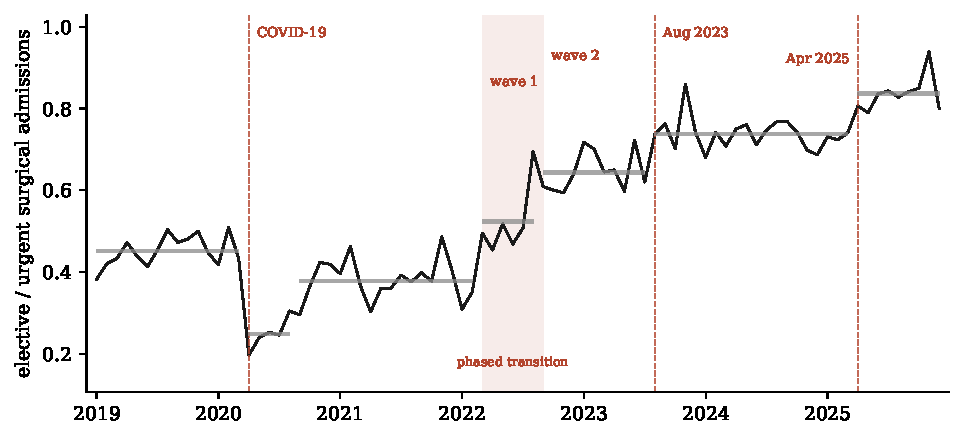
\includegraphics[width=\textwidth]{fig1_ratio_series.pdf}
\caption{Monthly elective-to-urgent surgical admission ratio, Goi\'as, 2019-2025.
Grey horizontal segments are within-regime means. Dashed vertical lines mark
the regime boundaries discussed in the text. The COVID-19 boundary at April
2020 is recovered by the changepoint procedure without being imposed.}
\label{fig:ratio}
\end{figure}

We locate regime changes using the PELT changepoint algorithm
\citep{killick2012} with an RBF cost, applied to the ratio series. To avoid
selecting break dates that we had already formed views about, we report the
procedure's output across penalty values rather than a single specification,
and we cross-check against a fixed-cardinality dynamic-programming search.
The procedure returns locations but not confidence intervals; see
Section~\ref{sec:limits}.

The procedure returns five boundaries at penalty 1.0 on the full sample: April
2020, September 2020, an unstable date in 2022 discussed below, August 2023 and
April 2025. Three of these have external referents. April and September 2020
bracket the pandemic suspension and recovery. The August 2023 boundary falls six months after the PNRF portaria, and the April 2025 boundary coincides with the start of PMAE disbursement. These are temporal coincidences; the analysis does not identify the effect of either programme.

The corresponding levels are as follows. In 2019 the state performed 3{,}896
elective and 8{,}625 urgent surgical admissions per month, a ratio of 0.452.
In the seven months from January to July 2022 it performed 3{,}812 elective and
8{,}564 urgent admissions per month, a ratio of 0.445. The state had returned
to its pre-pandemic elective volume and stopped there. From August 2022 to July
2023 elective volume rises to 5{,}986 per month, a ratio of 0.648, a level with
no precedent in the panel: the highest single month in 2019 reached 0.503, and
after August 2022 the series never again falls below 0.594. By 2025 the state
performs 8{,}013 elective admissions per month at a ratio of 0.811, roughly
double the 2019 level, while urgent volume over the same seven years rises by
only 15 per cent.

This rules out the most obvious alternative explanation. The increase is not
recovery from the pandemic, because recovery had already completed by early
2022 and the post-2022 level is not a return to any earlier level.

\subsection{Provider composition and the bed-day constraint}
\label{sec:provider}

Facilities are grouped by \texttt{TP\_GESTAO}, the CNES field recording which
authority administers the facility's SUS contract. Fifteen of 201 facilities
change this code during the panel, in every case from municipal to state and
never in the reverse direction: one in September 2019, five between April and
September 2020, seven in November 2021, one in April 2022 and one in July 2024.
One of these, CNES 5419662, is the April 2022 switch; it falls inside any
plausible pre-window and is excluded. We assign each remaining facility to the
status it held in August 2022, one month before the break, so that group
membership is pre-determined with respect to the 2022 change: 174 municipal-administered,
8 always state-administered, 13 transferred to state administration at some
earlier date, and 5 with no CNES record before September 2022, which together
contribute negligible elective volume and are reported rather than dropped
silently.

The label should not be read as ownership. Municipal administration in Goi\'as
covers a set of specialised private and philanthropic providers contracting with
SUS: the largest contributors of elective volume in this group are an oncology
hospital, a general private hospital, two Santa Casas, two ophthalmological
units and an orthopaedic hospital. State administration covers the purpose-built
state hospital network, including the two trauma centres, the women's hospital
and the paediatric hospital. Contract-administration authority is therefore
confounded with facility design and case portfolio, and the differences reported
below are properly read as differences between provider types rather than
between management regimes. Facility names and administration
codes are read from the June 2026 CNES establishment file, so a facility's group
is its status as recorded in that vintage rather than contemporaneously;
institutional type is stable across the panel for these categories.

\paragraph{Transfer status does not account for the growth.} Comparing the eight months
before the break (December 2021 to July 2022) with the eleven after it
(September 2022 to July 2023), facilities already state-administered throughout
grew elective volume by 176.7 per cent and facilities that had transferred at
some earlier date by 180.5 per cent, against 29.2 per cent for
municipal-administered facilities. Facilities that never switched grew as fast
as those that did. Status at the break predicts the magnitude of growth;
the date of transfer does not. This rules out a staggered event study on the
transfer date as the primary design.

\paragraph{The pre-break window is contaminated.} The state-administered share
of elective volume runs between 0.21 and 0.32 through 2019, collapses to 0.021
by June 2020 and recovers only erratically through 2021. The trough is far
deeper for state-administered facilities than for municipal ones, so a
comparison anchored on 2021--22 attributes differential pandemic recovery to the 2022 change. Re-baselined on 2019, state-administered volume grows by a factor of
2.15 and municipal-administered by 1.31, a ratio of ratios of approximately 1.6
rather than the sixfold gap implied by the contaminated window. The
state-administered share moves from 0.256 in 2019 to approximately 0.35 after
the break, a rise of 9.5 percentage points. All comparisons below use 2019 as
the counterfactual.

\paragraph{Throughput per bed tracks length of stay, and both gaps close.}
Merging monthly CNES bed records, municipal-administered facilities performed
more elective cases per surgical bed-month than state-administered ones in 2019,
1.38 against 1.04, a ratio of 1.32.\footnote{Surgical bed capacity is defined by
\texttt{CODLEITO} rather than \texttt{TP\_LEITO}, which omits obstetric-surgical,
paediatric-surgical and surgical intensive care beds and understates surgical
capacity by 31 per cent overall, asymmetrically across groups. The rate is
pooled: elective cases summed over facility-months with at least one surgical
bed, divided by surgical bed-months summed over the same cells. Facility-months
with beds and no elective cases enter with zero in the numerator, since dropping
them would condition the denominator on the outcome. The unweighted mean of
facility-level ratios runs the other way, at 0.75, 0.65 and 0.72 across the three
regimes, because the facilities with the highest rates are small.} That advantage
does not persist. By 2022--23 the two are level at 1.61 against 1.66, a ratio of
0.97, and over 2023--25 at 2.00 against 2.00, a ratio of 1.00. Both groups roughly
doubled their throughput per bed; the gap between them closed.

The closing is accounted for by length of stay, which is the quantity the model
actually consumes. Across elective admissions in calendar 2023, mean
\texttt{DIAS\_PERM} is 1.57 days at municipal-administered facilities
($n=49{,}793$) and 2.32 days at state-administered facilities ($n=28{,}581$), a
ratio of 1.48. That gap also narrows: measured over 2023--25 rather than calendar
2023 it is 1.64 days against 2.08, a ratio of 1.27. The two facts are one fact.
Cases per surgical bed-month equals elective occupancy of surgical beds times
thirty over mean length of stay, an identity that holds exactly on this
facility-month universe in all three regimes, so with elective occupancy of
surgical beds converging the throughput ratio is pinned by the length-of-stay
ratio. When the stay gap narrows, the throughput gap closes with it. The
pattern the rest of this subsection documents is therefore consistent with the
convergence and not only with a single cross-section.

Excluding the two largest facilities on each side by 2023 elective volume lowers
the length-of-stay ratio from 1.48 to 1.32, and the median of facility-level
means gives 1.59. The gap survives excluding the largest institutions on both
sides, which is what the comparison was for; it is not the creature of any single
institution, though the largest institutions do widen it.

Normalising on bed-days rather than cases removes the difference wherever one
exists. In 2019, when municipal-administered facilities performed 1.32 times as
many elective cases per surgical bed-month, they did so because their cases were
shorter and not because they turned beds faster; by 2023--25, with stays having
converged, the cases-per-bed difference has gone too. The comparison that varies
across the panel is cases per bed. The one that does not is the conserved
quantity: capacity is consumed in bed-days, and a case is a claim on it only
through its length of stay. That is what Section~\ref{sec:model} imposes.

\paragraph{Case mix explains none of the gap.} Reweighting state-administered
length of stay at municipal procedure weights, at the full ten-digit
\texttt{PROC\_REA} on 69 procedures with at least thirty cases on each side,
gives 2.05 against a municipal 1.35; reweighting municipal at state weights
gives 1.44 against a state 2.03. Both directions bracket the raw gap, so
composition contributes nothing. The gap decomposes instead into two distinct
margins. Twenty per cent of municipal elective admissions are same-day
discharges against 6.7 per cent of state-administered admissions, and the
procedures where this differs account for 35 per cent of the total gap. Among
procedures where both groups admit essentially every patient overnight,
state-administered stays remain 1.32 times longer, accounting for a further 56
per cent. The first margin is an admission-protocol difference, the second a
discharge-timing difference, and they carry different implications for capacity.

\paragraph{Complexity runs the wrong way.} The obvious alternative explanation
is that state hospitals are the referral tier and treat more complex cases. The
data invert this: 19.6 per cent of municipal elective admissions are coded high
complexity against 6.6 per cent of state-administered ones. The gap also widens
within each stratum, from 1.48 pooled to 1.58 among medium-complexity and 1.81
among high-complexity admissions. Standardising state-administered length of
stay on the municipal complexity distribution raises the ratio from 1.48 to
1.65. The pooled figure understates the difference because state-administered
facilities perform proportionally less high-complexity work, not more.

\paragraph{Capacity is unequally binding.} Total occupancy of SUS beds differs
sharply: 0.33 at municipal-administered facilities in 2023--25 against 0.79 at
state-administered ones, with facility-level medians of 0.15 and 0.84. Elective
occupancy of surgical beds, by contrast, converges, at 0.109 and 0.139 in the
same window, and both groups roughly doubled it relative to 2019. Both provider
types devote similar and similarly growing shares of surgical bed capacity to
elective work; what differs is the total load against which that share is drawn.
Total bed occupancy is lower at municipal-administered facilities, indicating more bed slack by this measure; the data do not establish the marginal operational cost of an additional elective case. This asymmetry, rather
than any difference in management quality, is what the assignment model in
Section~\ref{sec:model} must represent: machines are heterogeneous in bed-day capacity, in
the bed-day cost of a given procedure, and in how tightly that capacity binds.

Bed-days are attributed to the discharge \emph{compet\^encia} rather than spread
across the months an admission spans. This affects the occupancy series only;
every length-of-stay figure above is computed from record-level
\texttt{DIAS\_PERM} and is unaffected, as is the bed-day consumption parameter of
Section~\ref{sec:model}.

\paragraph{Where the capability appeared.} The capability that appeared between 2019 and 2023 (Appendix~\ref{sec:appb2}) is not distributed like the incumbent expansion. By group, the 284 pairs absent in 2019
divide into 191 pairs and 13{,}326 cases at
municipal-administered facilities, 43 pairs and 6{,}330 cases at always-state
facilities, and 42 pairs and 2{,}096 cases at transferred ones; the remaining 8 pairs
and 93 cases are at the two facilities of this section that fall outside the three groups
(3 pairs and 33 cases at a facility with no CNES record before September 2022, 5 pairs and 60 cases at CNES 5419662, the excluded April 2022 switch). They concentrate
in the high-availability subgroups: digestive system, annexed organs and abdominal wall (0407) carries 7{,}401 of
the new cases, genitourinary system (0409) 4{,}094 and musculoskeletal system
(0408) 3{,}490. The pattern of intervening activity holds within each: 78.1 per cent of the
0407 pairs, 80.0 per cent of the 0409 pairs and 78.9 per cent of the 0408 pairs
are active in some month of 2020 to 2022, carrying 97.2, 87.2 and 99.8 per cent
of their respective cases. The composition is worth naming. Within the 0409
volume the largest single procedure is total hysterectomy at 807 cases, followed
by postectomy at 615, vasectomy at 481 and tubal ligation at 414; male and female
sterilisation together account for 895 of the 4{,}094 cases, a distinct policy
fact from the growth in cholecystectomy that drives 0407. Most recorded tubal ligations in 2023 were at facilities that had also recorded the procedure in 2019 to 2022: of the 414 tubal ligations recorded at these facilities in 2023, 347 are at the sixteen of thirty-five that already performed the procedure between 2019 and 2022.

These facilities fall into two functional types, distinguished by the share of their
patients resident in the facility's own municipality. Local-demand units serve
their immediate population: the converted unit at CNES 9680977 draws 95 per cent
of its elective patients from its own municipality, a second An\'apolis facility
87 per cent and a Jata\'i unit 99 per cent. Regional referral nodes draw
predominantly from outside: the Centro Norte Goiano hospital 17 per cent, the
Luzi\^ania unit 12 per cent, and the paediatric state hospital 16 per cent. The
distinction matters for how the expansion is characterised. Two of the three
referral nodes are located in interior regions and lower the regional cost score for some of their catchments; the third is in the capital, so its patients travel
towards the centre rather than away from it. Added capacity at the centre and
decentralisation of capacity are separate phenomena and this expansion contains
both.

\subsection{Limitations}
\label{sec:limits}

Six limitations should be stated plainly, and two sources deserve a note. The health-region mapping used in one robustness row is the list of municipalities per region published on the SES-GO page ``Regi\~oes de Sa\'ude'' (18 regions, 246 municipalities, grouped into five macro-regions); it was read from that web page and not from the CIB resolution that established it, and the page lists 25 municipalities for one region but names 24 in one place, which we resolved by name matching to IBGE. The Entorno exclusion uses the 29 Goi\'as municipalities listed for the RIDE-DF in Lei Complementar n.\ 94/1998 as amended by Lei Complementar n.\ 163/2018 (index page of the C\^amara dos Deputados, which tags Planaltina as DF in its index; we read it as Planaltina de Goi\'as).

First, SIH records completed admissions and contains no information on waiting
time, queue registration date, or patients who never reached surgery. We observe
throughput, not service level, and cannot say whether the additional volume went
to the patients who had waited longest. A request for aggregate queue extracts
from the state regulation system is pending; were it to return, the objective in
Section~\ref{sec:model} could be stated in terms of waiting time rather than
travel.

Second, the break dates are estimated from the admission series and are not linked to any administrative act; the corresponding acts of SES-GO have not been read from the Di\'ario Oficial (one, Resolu\c{c}\~ao CIB n.\ 111/2021, is described in Section~\ref{sec:data}), so no break is attributed to an instrument.

Third, the break dates are point estimates. The changepoint procedure we use
returns locations but not confidence intervals, and we report its output across
penalty values rather than a single specification in place of a formal test. A
multiple-break test in the manner of \citet{bai1998} would place intervals on
the dates and has not been run.

Fourth, we cannot distinguish activation of latent capacity from silent capacity
expansion. The bed-day evidence shows the additional volume did not exhaust the constructed bed-day budget, but the corresponding measurement on staffing,
cases per surgeon-month from the CNES professional files, has not been made.

Fifth, bed-days are attributed to the discharge \emph{compet\^encia} rather than
spread across the months an admission spans. This affects the occupancy series
only. Every length-of-stay figure reported above is computed from the
record-level \texttt{DIAS\_PERM} field and is unaffected by the attribution rule,
as is the bed-day consumption parameter of Section~\ref{sec:model}, which is
estimated on the same field.

Sixth, facility-procedure pairs operate in bursts rather than switching on
permanently. Across the 84-month panel, 1{,}028 of 1{,}179 pairs record at least
one interruption of three consecutive months and 428 lapse and resume, so a
set-difference comparison between two calendar years conflates pairs new to the
record with pairs that resume after a lapse (the panel starts in 2019 and cannot show earlier spells). The same intermittency rules out dating entry at pair level: under
three defensible definitions of sustained activity --- first positive month,
first of three consecutive positive months, and first month whose three-month
rolling mean clears a floor --- only 31 to 39 per cent of pairs receive the same
entry month, and mean displacements between pairs of definitions run from six to twelve months. A staggered event study
on pair entry is therefore not available to us, since treatment timing would be
the identifying variation.

Two further checks belong to the analysis rather than to its interpretation. The geographic staggering reported in Appendix~\ref{app:timing} is measured at municipality level, whereas a
state regulation reform is rolled out along \emph{regi\~oes de sa\'ude}; the
crosswalk is not carried in the SIH reduced files. And the reliability filter
that defines our facility-level subset is a judgement about reporting behaviour,
not a measurement of it.

The results are a Goi\'as-specific diagnostic from SUS claims and should not be assumed to transfer to states with different facility, referral or regulatory structures.

\section{An assignment model of elective surgical capacity}
\label{sec:model}

The empirical sections establish three facts that determine the structure of any
model of this system. Capacity is consumed in bed-days rather than cases, and
procedures differ systematically in how many bed-days they consume. Facilities
differ in how tightly that capacity binds, with municipal-administered units
operating near a third of total bed occupancy and state-administered units near
four fifths. And elective surgery is regionally organised: over 2019 to 2025, 42.7 per cent of elective admissions occur outside the patient's municipality of residence, and
state-administered facilities draw 70.3 per cent of their elective patients from
outside their host municipality against 30.4 per cent at municipal-administered
facilities.

We therefore formulate the allocation of elective surgery in Goi\'as as a
capacitated assignment problem with a travel-penalised access objective, and use
it to ask a counterfactual question: given the observed facility set, the constructed bed-day budget and historical peak-volume caps, what allocation of elective cases would have
delivered the same volume at least travel cost, and how far was the observed
allocation from it?

At the reported optimum, aggregate utilisation of the constructed net surgical
bed-day budget is 0.132 in 2019, 0.178 in 2023 and 0.215 in 2025, and one, three
and six facilities use more than 95 per cent of it, while the peak-volume cap is
reached far more often. Section~\ref{sec:capbind} reports this at the reported
optimum, and Section~\ref{sec:capnull} tests how much of it survives across
optima of equal cost and against counting noise; less survives than the reported
optimum suggests. Section~\ref{sec:decomp} describes how the attainable frontier moved: most of the improvement between
2019 and 2023 comes with the arrival of facility-procedure pairs absent in 2019 and the caps they carry,
though the split between options and capacity depends on the order of steps. Because the set of pairs itself changes, the fixed-machine-set restriction stated in
Section~\ref{sec:fixed} is a substantive question rather than a caveat.

\subsection{Sets and parameters}
\label{sec:sets}

Let $I$ index municipalities of residence, $J$ index facilities, and $P$ index
procedure subgroups at the four-digit SIGTAP level. Residents of municipalities
outside Goi\'as account for approximately 0.7 per cent of elective admissions and
are dropped, leaving $|I| = 246$. In 2019 and 2023, $|J| = 131$ facilities have
positive elective volume and non-zero net bed-day capacity; in 2025 there are
145. In every year $|P| = 16$.

\paragraph{Scope of the observed baseline.} The observed mean travel cost the
optimum is compared against is computed on admissions at facilities in $J$:
74{,}832 of the 79{,}247 in-state elective admissions of 2023, or 94.4 per cent.
The 5.6 per cent excluded had a higher mean cost index than the records retained, a mean of
1.003 index units against 0.846, so scoring the same optimum against the
all-records observed mean raises the estimated gap to 31.3 per cent rather than
the 30.6 per cent reported. The reported figure is the conservative one.

Demand $d_{ip}$ is the count of elective admissions of procedure type $p$ by
residents of municipality $i$ in the period. We treat observed admissions as a
lower bound on demand, since SIH records completed admissions and is silent on
patients who never reached surgery; Section~\ref{sec:limits} states what this
does and does not permit us to claim.

Throughout, $d_{ip}$, $B_j$ and $\kappa$ are monthly quantities (annual totals divided by twelve). Capacity $B_j$ is facility $j$'s surgical bed-day endowment: SUS surgical beds
from the CNES bed file multiplied by 30 days per month (calendar days per month, 30.4 on average, move the 2023 gap by +0.5 points), net of the bed-days
consumed by urgent surgical admissions at that facility. Netting all
non-elective bed-days, including clinical, obstetric and intensive care, against
surgical beds alone drives a third of facilities to zero capacity and is not the
correct pairing; numerator and denominator must both be surgical. Bed-day
consumption $\lambda_{jp}$ is the mean length of stay of procedure type $p$ at
facility $j$, estimated on observed admissions and shrunk toward the
procedure-level mean with weight $K=30$ where facility-procedure cell counts are
small.

Travel cost $c_{ij}$ is ordinal rather than metric, taking value $0$ if facility
$j$ lies in municipality $i$, $1$ if it lies in $i$'s IBGE immediate region,
$2$ if in $i$'s intermediate region, and $3$ otherwise. This uses IBGE immediate and intermediate geographic regions, which resemble but are not the CIB health regions (regi\~oes de sa\'ude) on which SUS referral agreements are written, and avoids
imputing road distances that the administrative data does not contain.

\paragraph{Metric robustness.} Replacing the ordinal cost with great-circle
distance between municipal seats raises the estimated gap rather than lowering
it, to 36.6 per cent in 2019, 39.7 in 2023 and 31.6 in 2025, against 28.8, 30.6
and 29.1 on the ordinal. The two constructs also largely agree on which
allocations are good. The ordinal-optimal 2019 solution carries 38.8 km per case
against a metric optimum of 31.5 and an observed 49.6; the metric-optimal
solution carries 0.634 index units against an ordinal optimum of 0.595. We
report the
ordinal figure throughout because it follows the IBGE regional hierarchy, which
resembles the health regions on which SUS referral is organised (official health
regions are a robustness row in Table~\ref{tab:measure}), and because it is the more conservative of the two.
Great-circle distance is itself a proxy: it ignores the road network, which in
interior Goi\'as can make actual travel substantially longer than the straight
line.

\subsection{Decision variables and formulation}
\label{sec:formulation}

Let $x_{ijp} \geq 0$ be the number of elective cases of type $p$ from
municipality $i$ performed at facility $j$, and let $u_{ip} \geq 0$ be unmet
demand. The program is

\begin{align}
\min_{x, u} \quad & \sum_{i,j,p} c_{ij}\, x_{ijp} \;+\; \pi \sum_{i,p} u_{ip} \label{eq:obj}\\
\text{s.t.} \quad & \sum_{j} x_{ijp} + u_{ip} = d_{ip} && \forall i, p \label{eq:demand}\\
& \sum_{i,p} \lambda_{jp}\, x_{ijp} \leq B_j && \forall j \label{eq:capacity}\\
& \sum_{i} x_{ijp} \leq m\,\kappa_{jp}, \quad \sum_{i,p} x_{ijp} \leq m\,\kappa_{j} && \forall j, p \label{eq:cap}\\
& x_{ijp} = 0 && \forall (j,p) \notin S \label{eq:scope}\\
& x_{ijp}, u_{ip} \geq 0. \nonumber
\end{align}

Constraint~\eqref{eq:demand} conserves demand. Constraint~\eqref{eq:capacity} is
the bed-day budget: this is where the length-of-stay result enters, since a
facility that treats a given case mix with longer stays exhausts its budget at
fewer cases. Constraint~\eqref{eq:cap} is the historical peak-volume cap,
described below. Constraint~\eqref{eq:scope} restricts each facility to the
procedure types it has been observed to perform, with the scope set $S$ taken
from observed activity in the estimation window rather than assumed. The scope
set closes 73 per cent of the assignment space, counted over the full
$|I| \times |J| \times |P|$ grid of 515{,}616 triples; the number of facilities
performing a given subgroup ranges from 5 to 97. The program is built only over
demand cells that are non-empty, so the variable count reported in
Section~\ref{sec:modelresults} is smaller again.

\paragraph{The peak-volume cap.} $\kappa_{jp}$ and $\kappa_{j}$ are facility $j$'s
peak 3-month average volume in the estimation year, for procedure $p$ and in total. This is
a historical high-water mark, a lower bound on what the unit has delivered and not a measured
ceiling on what it can deliver (Section~\ref{sec:capnull}); we call it a cap because the program
imposes it as one. The natural construction is the largest monthly caseload observed in the estimation year.
Bounding facility throughput by observed case volume in this way is in the spirit of
\citet{vogel2022}, who constrain each hospital to a multiple of its base-year
volume when simulating minimum volume regulation in the German hospital sector;
our multiplier ladder in Table~\ref{tab:modelrobust} plays the same role as
their $v_{\max}$. Section~\ref{sec:data} documents batch reporting in SIH, and a facility that
bills two months of work in one produces a maximum that overstates what it can
do. In 2023, 37 of the 136 facilities with positive elective volume report
interleaved zero months within their span, carrying 12.4 per cent of elective
volume, and their ratio of single-month maximum to three-month rolling maximum
is 1.53 against 1.21 for the rest. The count is 136 rather than the $|J| = 131$
of Section~\ref{sec:sets} because five facilities with elective volume in 2023
have no net surgical bed capacity once urgent consumption is deducted, and are
not carried into the program. We therefore define $\kappa$ as the largest
three-month rolling mean of monthly volume, applied uniformly to every facility
rather than only to those classified as batch reporters, so that the rule does
not condition on a classification we constructed. This tightens total cap
capacity by 20 per cent relative to the single-month maximum and lowers the
reported gaps; the single-month rule is reported as a robustness row.

Pairs whose rolling mean falls below half a case per month are given a floor of
$0.5$, so that a pair observed to exist is not assigned a cap of effectively
zero. The floor is a construct rather than a measurement, and pairs subject to it
are excluded from every pair-level count reported below. They are not a small
group: of the pairs carrying positive flow at the optimum, 116 of 532 are floored
in 2019, 111 of 601 in 2023 and 100 of 663 in 2025, between a sixth and a fifth
of the option set in use. Their share of served volume is small, falling from
1.3 per cent in 2019 to 0.7 and then 0.5, because a floored pair is by
construction one that carries almost no volume. Their shadow prices are not
small, however, and Section~\ref{sec:capbind} reports the consequence: because
the floor is a construct rather than a measurement, a floored pair at its cap
should not be read as a facility at the limit of what it can do.

Every pair-level share reported below therefore has as its denominator the pairs
that carry positive flow at the optimum and are not floored: 416 of 563 scope
pairs in 2019, 490 of 637 in 2023 and 563 of 704 in 2025. The gap between scope
and use is the pairs the optimum declines to employ at all, 31, 36 and 41
respectively. A pair is counted as binding when it carries more than 95 per cent
of its cap.

\paragraph{What the peak-volume cap restricts.} Equation~\eqref{eq:cap} has two
rows, and they do different work. Dropping the pair row and retaining only the
facility total isolates them. With no peak-volume constraint at all the gap is
50.4 per cent in 2019, 56.1 in 2023 and 56.4 in 2025. Imposing only the facility
total takes it to 35.5, 39.4 and 40.1. Imposing the pair row as well takes it to
28.8, 30.6 and 29.1. The first step, worth 14.9, 16.7 and 16.3 points, is the effect of the facility-total cap. The
second, worth 6.7, 8.8 and 11.0 points, is the effect of the pair-level cap. The facility-total step is the larger throughout, but the pair-level step grows across the panel, from 31 to 35 to 40
per cent of the combined restriction. Both rows therefore restrict the benchmark, and the pair row's share grows across the panel.

This matters for how a shadow price on $\kappa_{jp}$ should be read. Where the
facility total also binds, relaxing one pair's cap moves volume within the
facility rather than adding to it, so the pair's dual is not the value of new
capability at that pair alone. That is the majority case: of the pairs carrying a
positive dual, 62 per cent in 2019, 55 in 2023 and 79 in 2025 sit at a facility
whose total cap is also binding. Section~\ref{sec:placement} conditions on this
rather than ranking on the raw dual.

The penalty $\pi$ prices unmet demand against travel. It is the only parameter
in the program with no empirical referent: the shrinkage weight $K = 30$, the
$0.5$ floor and the three-month rolling window are also chosen rather than
estimated, but each is a construction applied to observed quantities, whereas
$\pi$ is a price the data does not contain. Where the program serves all demand, $\pi$ does not enter the
solution at all. Where capacity binds, we report results across $\pi \in
\{4, 6, 10\}$ and show in Section~\ref{sec:decomp} that the ordering of
configurations is invariant over that range.

\paragraph{Comparing configurations that leave demand unmet.} Mean travel cost
over served cases is not comparable across configurations with different unmet
volume. When capacity binds, the program chooses which demand to leave unserved,
and it drops the cells whose nearest permitted facility is farthest; the served
pool is then a closer, selected subset and its mean travel falls mechanically.
Tightening capacity can therefore appear to improve routing. We report instead
an adjusted cost that charges unmet demand at $\pi$ and divides by total rather
than served demand,
\[
\bar{c}^{\,\text{adj}} \;=\; \frac{\sum_{i,j,p} c_{ij} x_{ijp} \;+\; \pi \sum_{i,p} u_{ip}}{\sum_{i,p} d_{ip}},
\]
which is the objective value per unit of demand and is defined on the same
denominator in every configuration. Where unmet demand is zero the two measures
coincide.

\subsection{What the model does and does not treat as fixed}
\label{sec:fixed}

The machine set is fixed within a period, and this is the model's central
restriction rather than an incidental one. Appendix~\ref{sec:appb2} establishes that the set of facility-procedure pairs changes from year to year: 284 pairs
present in 2023 are absent in 2019 and 192 go the other way, and most of the 284
had earlier activity in the record. A model that cannot open or close pairs therefore
cannot represent the change in the set of pairs through which this system expanded. We
solve the model period by period on the capacity that existed in that period,
and read the within-period gap as the distance between the observed allocation and the benchmark for that period's pairs and caps.
Section~\ref{sec:decomp} then relaxes the restriction across periods to
describe how the frontier moved.

Urgent demand is not modelled explicitly. It enters through $B_j$, which is net
of the bed-days consumed by urgent surgical admissions at each facility in the
period. This is why urgent use matters for the solution rather than merely describing it: a facility with heavy urgent surgical use contributes a smaller bed-day budget than its bed count suggests.

\subsection{Results}
\label{sec:modelresults}

We solve the program on three years: calendar 2019, the last full pre-pandemic
year and the baseline the empirical sections establish as the appropriate
counterfactual; calendar 2023; and calendar 2025, the most recent complete year
in the data. The 2019 instance has 246 municipalities of residence, 131
facilities and 16 procedure subgroups, giving 99{,}025 assignment variables over
2{,}294 demand cells; the 2025 instance is the largest, with 145 facilities and
704 facility-procedure pairs in scope. All three solve to optimality in
seconds.

The observed 2019 allocation carries a mean travel cost of 0.835
index units per elective case. The unconstrained optimum delivers identical
volume, with no unmet demand, at 0.414: a reduction of 50.4 per cent. This
figure should not be the headline, because with bed-days slack almost everywhere
the program is free to route demand to any facility within its observed scope,
including facilities that performed the procedure only a handful of times.
Table~\ref{tab:modelrobust} therefore reports the ladder of peak-volume caps.

\begin{table}[t]
\centering
\caption{Optimal mean travel cost under increasingly tight caps on facility
throughput. The cap restricts each facility to a multiple of its largest
three-month rolling mean monthly elective caseload in the estimation year. All
specifications serve the full observed volume with zero unmet demand, so the
adjusted and served-only costs coincide throughout.}
\label{tab:modelrobust}
\begin{tabular}{lrrrrrr}
\toprule
& \multicolumn{2}{c}{2019} & \multicolumn{2}{c}{2023} & \multicolumn{2}{c}{2025} \\
\cmidrule(lr){2-3}\cmidrule(lr){4-5}\cmidrule(lr){6-7}
Specification & Cost & Reduction & Cost & Reduction & Cost & Reduction \\
\midrule
Observed allocation & 0.835 & --- & 0.846 & --- & 0.906 & --- \\
Unconstrained optimum & 0.414 & 50.4\% & 0.372 & 56.1\% & 0.395 & 56.4\% \\
Cap at 2$\times$ historical peak & 0.513 & 38.6\% & 0.474 & 43.9\% & 0.518 & 42.8\% \\
Cap at 1.5$\times$ historical peak & 0.542 & 35.1\% & 0.507 & 40.1\% & 0.551 & 39.2\% \\
Cap at 1$\times$ historical peak & 0.595 & 28.8\% & 0.587 & 30.6\% & 0.642 & 29.1\% \\
\midrule
\multicolumn{7}{l}{\emph{Robustness: single-month maximum in place of three-month rolling mean}} \\
Cap at 1$\times$ historical peak & 0.537 & 35.7\% & 0.509 & 39.9\% & 0.559 & 38.2\% \\
\bottomrule
\end{tabular}
\end{table}

The result to take is the 1$\times$ row. Constraining every facility to do no more per month than its highest recorded three-month average, the
same volume of elective surgery could have been delivered in 2019 at 0.595
index units per case against an observed 0.835, a reduction of 28.8 per cent. The observed allocation respects the caps by construction but exceeds the bed-day budget at 1, 2 and 4 facilities, so it is not strictly a feasible point of the program and the sign of the gap is not guaranteed by construction; the gap measures distance under the program's rules, and we offer no threshold for what size would indicate a problem. This specification needs no outside estimate of capacity: each facility is held to its own
peak 3-month average volume. It does assume that this historical peak is a feasible level for the unit. Just over half of the
unconstrained gain survives the binding cap: 0.240 of 0.421 index units in
2019, and 54.6 and 51.7 per cent of it in 2023 and 2025.

The later columns are the more striking ones. The observed mean index did not fall
across the panel; it rose, from 0.835 in 2019 to 0.846 in 2023 and 0.906 in
2025, while elective volume more than doubled. The optimum under the
cap moves little against that: 0.595, 0.587, 0.642. The point estimates of the
gap are close, 28.8, 30.6 and 29.1 per cent, and the differences between years
are not distinguishable from zero (Section~\ref{sec:uncertainty}); the intervals are too
wide to establish that the gap was constant. Municipal rankings of excess ordinal cost
are correlated across years, at 0.68 to 0.74 (Section~\ref{sec:flows}). We do not
attribute the absence of a detectable change to any reform.

Two qualifications belong with the number. Travel cost here is an ordinal index (0 to 3), not kilometres and not a count of region
crossings, so a ratio of its means has no distance interpretation; the gap is a statement about
the index, and its level depends on the coding (Section~\ref{sec:capnull}). And the model routes on procedure
subgroup and observed scope alone; it does not observe surgeon subspecialty,
equipment, or the case-volume thresholds that clinical governance may impose
within a subgroup. Some part of the observed cost index is therefore a constraint the
data does not record. The peak-volume cap absorbs the facility-level version of
this concern but not the procedure-specific version.

\subsection{How the attainable frontier moved between 2019 and 2023}
\label{sec:decomp}

The two years differ in three respects that the ladder above cannot separate:
demand is larger in 2023, capacity is larger, and the set of facility-procedure
pairs is larger, 637 against 563. We separate them by solving four
configurations, each combining a demand year with an option set and a capacity
vintage. Table~\ref{tab:decomp} reports them.

\begin{table}[t]
\centering
\caption{Decomposition of the 2019--2023 frontier. Adjusted cost charges unmet
demand at $\pi$ and divides by total demand; see Section~\ref{sec:formulation}.
Configurations A and D serve all demand, so their adjusted and served-only costs
coincide.}
\label{tab:decomp}
\begin{tabular}{llrrrr}
\toprule
& Configuration & Options & Served-only travel & Adjusted cost & Unmet \\
\midrule
A & 2019 demand, 2019 options, 2019 capacity & 563 & 0.595 & 0.595 & 0.0\% \\
B & 2023 demand, 2019 options, 2019 capacity & 563 & 0.725 & 1.823 & 20.8\% \\
C & 2023 demand, 2019 options, 2023 capacity & 554 & 0.775 & 1.375 & 11.5\% \\
D & 2023 demand, 2023 options, 2023 capacity & 637 & 0.587 & 0.587 & 0.0\% \\
\bottomrule
\end{tabular}
\end{table}

Configuration C carries 554 options rather than A and B's 563 because the option
set is intersected with the capacity vintage it is solved against: five
facilities with 2019 elective volume have no net surgical bed capacity in 2023,
removing fourteen pairs, while one facility with 2019 volume and no 2019 net
capacity acquires some by 2023, adding five.

Configurations C and D differ only in which facility-procedure pairs are permitted: 554 against 637, on identical
demand and identical capacity. With the 2019 pairs 11.5 per cent of the 2023 demand is unserved and travel over the cases served is 0.775; with the 2023 pairs
all demand is served at 0.587. We do not attribute the change between options and capacity. The pairs absent in 2019 and the caps they carry arrive together,
and any split depends on the order of steps and on the penalty $\pi$ that prices unmet demand; the table reports served-only travel and the unmet share separately for that reason.

The option set did not simply accumulate. Between 2019 and 2023 the state gained
284 facility-procedure pairs and lost 192, a gross churn of 476 against a net
change of 92, both counted at the four-digit level at which the model routes.
This strengthens rather than weakens the comparison: configuration C is solved on
the 2019 option set including the pairs that later disappeared, so the
improvement from C to D is net of the exits, not gross of them.

Configuration B adds the 2019 capacity vintage to the 2019 option set and leaves
a fifth of 2023 demand unserved. The 2019 option set was generous relative to
2019 volume, in the sense that configuration A serves all demand with just over
half of the unconstrained gain still available, and binding relative to 2023
volume.

The ordering A $\approx$ D $<$ C $<$ B holds at $\pi = 4$, $6$ and $10$.
Configurations A and D serve all demand, so $\pi$ does not enter them.
Configuration B's allocation is identical at all three values and only the charge
on a fixed quantity of unmet demand changes. Only configuration C reallocates,
with unmet demand moving from 11.8 to 11.5 to 11.4 per cent as $\pi$ rises
through 4, 6 and 10, and configuration B's from 21.2 to 20.8. The decomposition
is therefore not an artefact of the penalty.

\subsection{Beds and the peak-volume cap at the reported optimum}
\label{sec:capbind}

Table~\ref{tab:decomp} shows that with the 2023 pairs and caps all 2023 demand is assigned. The ratio of aggregate cap to demand did not rise.
Capability capacity, the sum over facilities of the rolling-mean cap, rose 64.9
per cent between 2019 and 2023 against a 70.7 per cent rise in demand.
Aggregate peak-volume cap exceeded demand by a factor of 1.368 in 2019, 1.321 in 2023
and 1.160 in 2025. Surgical bed-days rose 20 per cent between the first two
years. At the pair level, 233 of 416 facility-procedure pairs bind at the 2019
optimum, 249 of 490 in 2023 and 339 of 563 in 2025, carrying 54.5, 46.0 and 54.4
per cent of served volume. The option set expanded at approximately the rate
demand did through 2023 and more slowly thereafter, so the ratio of aggregate peak-volume cap to demand falls rather than rises: by 2025
the cap exceeds demand by 16 per cent against 37 per cent in 2019. Section~\ref{sec:capnull}
asks what the fall consists of.

Two utilisation measures appear below and they are not the same quantity.
\emph{Aggregate} bed utilisation is state-wide bed-days used over state-wide
bed-days available, and is the series reported in this subsection and in Section~\ref{sec:capnull}. \emph{Mean facility utilisation} is the
unweighted mean of facility-level ratios over a named subset of facilities, and
is always smaller here because the facilities holding the most spare capacity are
small.

The two constraints bind on almost disjoint sets of facilities. In 2023 three
facilities use more than 95 per cent of their bed-day budget, and those three operate at
0.58 of their peak-volume cap. At the reported optimum 77 facilities are at their cap, with mean
facility utilisation 0.116, and hold 26{,}269 unused surgical bed-days per month
between them, against 10{,}902 bed-days consumed per month by all 131 facilities
in the solution. The two figures have different denominators and their ratio is
not a utilisation rate; aggregate bed utilisation in the same solution is 0.178.
In 2019 one facility reaches its bed-day budget, at 0.41 of its peak-volume cap,
while 79 reach their peak-volume cap at mean facility utilisation 0.115 and hold
23{,}821 spare bed-days. In 2025 six facilities are bed-bound at 0.63 of their
peak-volume cap, while 105 of 145 are at their peak-volume cap at mean facility
utilisation 0.149 and hold 31{,}309 spare bed-days.

At the reported optimum no facility is both bed-bound and at its peak-volume cap in 2019 and 2023, and
144 of 145 facilities are not both in 2025. The exception is CNES 2382474 in S\~ao Lu\'is de Montes Belos, which in the
2025 solution reaches bed utilisation 1.000 and cap use 0.985 simultaneously.
The 2025 overlap is not a trend: in the 2019 optimal face a facility can already be both bed-bound and at cap
(Section~\ref{sec:capnull}), so an overlap appearing in 2025 at this vertex does not mark a leading edge. The ratio of aggregate peak-volume
cap to demand falls from 1.368 to 1.160 and state-wide bed utilisation moves from 0.132 to 0.178 to 0.215, and the facilities at their cap
are, at the reported optimum, mostly ones with bed-days to spare. The share of pairs that bind is not monotone, at 56.0, 50.8 and 60.2 per cent.
Beds, counted at full occupancy, are not scarce at any of the three dates in this program; operating-room sessions, surgeons and
anaesthetists are not modelled.

Read with Section~\ref{sec:results}, this describes the expansion without identifying its cause. Bed utilisation rose only from 0.13 to 0.21
while elective volume more than doubled, and routing showed no detectable improvement. What changed in the record is the set of active facility-procedure pairs,
most of them pairs with earlier activity in 2020 to 2022 (Appendix~\ref{sec:appb2}).
Whether the right response is to place capability or to change how existing capability is used is a policy question this model does not answer.

\subsection{What the peak-volume cap is, and what survives}
\label{sec:capnull}

The cap $\kappa$ is a peak: the largest 3-month average of a unit's own monthly volume in the estimation year. A maximum over
windows exceeds the mean mechanically, so several statements about it need a test against what noise alone would produce. This
subsection reports those tests. A record of when each rule was written relative to its results is in the repository (\texttt{dist/sprint/PREREG\_CHRONOLOGY.md}); only some were committed before their results existed.

\paragraph{The at-cap count is not identified.} The program's optimum is a face, not a point: many allocations have the same
cost. We searched that face (cost within $10^{-9}$ of optimal; a margin of $10^{-4}$ of the cap for a facility to count as at cap; 200 seconds per
search; every count quoted in a row comes from one solution, and no row constraint was violated by more than $10^{-14}$ in relative terms). The number of facilities using more than 95 per cent of their
peak-volume cap has a proved minimum of 34 of 131 in 2019, 44 of 131 in 2023 and 64 of 145 in 2025. The largest value found is 101, 107 and 115, with upper bounds of
113, 108 and 131 that the solver did not close. At 90 per cent the proved minimums are 39, 52 and 69, and at 99 per cent 31, 43 and 53. At the reported optimum (the stored solution) the counts are 79, 77 and 105; a fresh solve of the same program lands on another vertex with 72, 75 and 103, which is the non-uniqueness at work. Bed-bound facilities (more than 95 per cent of the
bed-day budget) range from 0 to 2 in 2019 (proved), from 2 to at least 4 (upper bound 5) in 2023 and from 4 to at least 7 (upper bound 9) in 2025, against 1, 3 and 6 at the reported optimum (1, 3 and 5 at the fresh solve). Statements about how many facilities ``are at their cap'' are therefore statements about one optimum among many. The unused surgical
bed-days at facilities at cap are at least about 9{,}700 (2019) and 12{,}100 (2023) at some optimum; we did not establish their upper range at these settings, so the 26{,}269 bed-days
quoted earlier for 2023 is the value at the stored solution only.

\paragraph{Disjointness.} At the reported optimum the two constraints bind on disjoint sets of facilities in 2019 and 2023 and overlap at one facility in 2025. Across the optimal
face, an overlap of one facility is attainable in 2019 (proved) and of two in 2025 (found; the solver could not rule out more, with an upper bound of five). In 2023 no overlap
was found, but the search did not prove that none exists (upper bound two within the time limit). Disjointness is therefore a statement about the reported optimum and not about
the face. How informative it is against chance depends on the vertex: with $K$ bed-bound and $n$ at-cap facilities among $N$, the probability under random assignment of an overlap as small as the one
observed ranges across the extreme vertices from 0.23 to 0.80 in 2019, 0.03 to 0.19 in 2023 and 0.001 to 0.17 in 2025 (0.40, 0.07 and 0.006 at the reported optimum). In 2019 the minimum number of
bed-bound facilities across the face is zero, so the claim can be vacuous there.

\paragraph{The cap test.} If caps bind, units at their cap in year $t$ should be exceeded less often in year $t+1$ than a
stationary system would exceed them. Among facilities at cap, 51.3 per cent (2023 to 2024) and 52.4 per cent (2024 to 2025) have a
larger peak the next year. Rebuilding the peak, re-solving the program and redefining ``at cap'' on 200 simulated stationary years,
that rate is 45.9 per cent (95 per cent range 35.5 to 53.8; $p = 0.13$) and 44.2 per cent (36.4 to 53.6; $p = 0.05$) when each unit's
months are Poisson, and 47.9 per cent (36.3 to 58.1; $p = 0.24$) and 47.7 per cent (37.5 to 56.9; $p = 0.18$) when each facility's
months are resampled from its own observed months, which keeps its overdispersion. The observed rates are inside the null range. This is a
low-power non-rejection: it is not evidence that the cap binds and not evidence that it does not. The contrast between the at-cap and not-at-cap rates
(observed $+0.17$ and $+0.21$) is also inside the null range (Poisson $+0.04$ with range $-0.28$ to $+0.34$, $p = 0.21$, and $-0.14$ with $-0.60$ to $+0.40$, $p = 0.07$; resampling $+0.07$
with $-0.11$ to $+0.24$, $p = 0.13$, and $+0.07$ with $-0.11$ to $+0.25$, $p = 0.06$). Restricting to the 43 facilities that are at cap in every optimum of equal cost in 2023 (a fixed set, so the null does not simulate the
selection), 55.8 per cent exceed their cap in 2024 against a null of 43.4 per cent (27.9 to 58.1; $p = 0.07$). The size of the exceedance is larger than the resampling null produces
(a median of 71 and 54 per cent of the cap, against 19 and 21 per cent), but this test does not separate growth in demand from a cap that was never binding, and we
claim neither. Where the CNES count of registered surgeons rose, at-cap facilities exceeded their cap in 79 and 63 per cent of cases against null rates of about 48 and 50 per cent; we treat this as
exploratory and unidentified: it is a registration count, it does not control for facility growth, and the urgent-volume placebo shows no such excess.

\paragraph{What the ratio of cap to demand contains.} The aggregate ratio of caps to demand (1.368, 1.321, 1.160) is not slack in
the sense of unused capacity. The sum of caps over the sum of mean volume at the same facilities is 1.37, 1.40 and 1.27, and the expected maximum 3-month mean of twelve Poisson months at those means would alone give a
ratio of about 1.09 (the one floor we use), so about a quarter of the excess over one exists by construction. We tested whether the fall in the ratio reflects flatter monthly series, with a rule stated for the
2019-to-2025 comparison: the volume-weighted peak-to-mean ratio net of that floor, over the 96 facilities present in both years, changes by $-0.07$ (95 per cent facility-bootstrap interval $[-0.15, +0.01]$). The interval includes
zero, so the explanation ``flatter months'' is not supported. The 2019-to-2023 fall coincides with falling coverage (the facilities in the model account for 100, 94 and 91 per cent of demand). A 2023-to-2025 contrast, chosen after seeing the
full-period result, gives $-0.12$ ($[-0.22, -0.05]$) and is exploratory. We do not describe the fall as a tightening of capacity.

\paragraph{Measurement choices.} Table~\ref{tab:measure} reports the gap when the inputs are rebuilt differently. The gap is robust
to defining months by discharge date and, in 2019 and 2023, to the estimation window. It is not robust to the cost coding (an
ordinal index counting municipality as a step: 29 to 31 per cent; boundary crossings only: 37 to 41 per cent), to the bed-day
definition (netting all admissions against all inpatient beds admits more facilities and gives 29, 37 and 40 per cent) or, in 2025, to
the window (25 per cent for July to June). Bed utilisation stays low under every definition (0.06 to 0.22, each definition solved afresh) and at most one facility is bed-bound when all admissions are netted against all inpatient beds, but the bed row is not inert: dropping it raises the gap by 0.0, 3.5 and 2.4 points (2019, 2023, 2025) because 1, 3 and 5
facilities would then exceed their bed-day budget, while replacing the shrunk stay lengths by facility-procedure means leaves the gap unchanged (0.0, 0.0 and $-0.1$ points). Beds are slack in aggregate and bind at a few facilities.
Observed elective bed-days exceed the budget at 1, 2 and 4 facilities. Batch
reporting is not the main source of month-to-month variation: defining months by discharge date lowers the number of facilities with
interleaved zero months only from 45 to 38 and from 36 to 31, so the rolling three-month mean is a smoother, not a correction for a
processing artifact. Zone size matters in the same direction. Aggregating origins to the IBGE immediate region, with cost 0 for a facility in the same region, is the same program as the boundary-crossing recoding (cost then depends only on the origin's region) and gives 37.1, 39.9 and 41.0 per cent; aggregating to the IBGE intermediate region to 38.1,
47.1 and 51.0, because a coarser zone hides which patients already travel within their zone; the gap is zone-dependent by more than five
points at every zone size. The gap computed against all in-state records, rather than records at model facilities, is 28.8, 31.3 and 29.0
per cent, within 0.7 points of the headline.

\paragraph{The gap depends on the cap.} The cap is built from the same months it constrains and is a peak, so each pair is given
headroom of peak over mean. Replacing the peak with the unit's annual mean volume (the fixed-marginal benchmark of the
excess-commuting literature) leaves almost nothing to reallocate in 2019, a gap of 6.2 per cent with 0.3 per cent of demand unserved; in 2023 the gap is
22.7 per cent with 7.3 per cent unserved and in 2025 29.6 per cent with 9.8 per cent unserved, so those are not like-for-like. Deflating the peak by
the expected excess of the maximum of twelve Poisson months over their mean gives 22.7, 24.0 and 24.8 per cent, 6.0, 6.5 and 4.3 points below the
headline. The headline gap is therefore partly headroom that a peak always has over a mean, and is reported with this bracket.
Bed utilisation is not an artifact of the cap: it is 0.12, 0.178 and 0.198 at the 2$\times$ cap and 0.129, 0.188 and 0.199 with no cap (2019, 2023,
2025), against 0.132, 0.178 and 0.215 at 1$\times$. Across the optimal face it ranges from 0.122 to 0.166, 0.165 to 0.217 and 0.206 to 0.238.


\begin{table}[t]
\centering
\caption{The gap (per cent) under alternative constructions of the inputs; reported-optimum values. The July-to-June window needs the
preceding year, so 2019 is not available; discharge-month results for 2025 are omitted because the files that would complete December
2025 do not exist.}
\label{tab:measure}
\small
\begin{tabular}{p{0.60\textwidth}rrr}
\toprule
Construction & 2019 & 2023 & 2025 \\
\midrule
Paper (month of processing, calendar year, ordinal cost) & 28.8 & 30.6 & 29.1 \\
Month of discharge (DT\_SAIDA) & 29.1 & 29.0 & --- \\
July-to-June window & --- & 30.5 & 25.2 \\
Actual days per month in the bed budget & 28.8 & 31.1 & --- \\
All admissions netted against all inpatient beds & 28.9 & 36.9 & 40.3 \\
Boundary-crossing cost (0/0/1/2); same as origin zone = IBGE immediate region & 37.1 & 39.9 & 41.0 \\
Origin zone = IBGE intermediate region (cost 0/1) & 38.1 & 47.1 & 51.0 \\
Baseline over all in-state records & 28.8 & 31.3 & 29.0 \\
Residents of the 29 RIDE-DF Entorno municipalities excluded & 29.6 & 32.3 & 28.5 \\
Official health regions (SES-GO, 18) replace IBGE regions in the cost & 30.7 & 35.1 & 30.7 \\
Origin zone = health region (cost 0/1/2) & 39.0 & 47.5 & 43.7 \\
Origin zone = health macro-region (cost 0/1) & 44.3 & 51.3 & 54.6 \\
\bottomrule
\end{tabular}
\end{table}

\subsection{Where the gap falls}
\label{sec:flows}

The aggregate gap conceals an allocation. The 2023 optimum assigns 2{,}908
origin-facility-procedure flows, and ranking municipalities of residence by excess ordinal cost, the difference between observed and optimal mean cost weighted by
served volume, locates the gap geographically. Total excess is 1{,}668 cost
units per month across 246 municipalities. The fifteen largest origins carry 44.6
per cent of net total excess (44.3 per cent of the sum of the positive entries, the denominator
used when negative entries are set aside).

Two properties of this measure should be stated before it is read. Excess weights
each municipality by the volume the optimum assigns it, while the aggregate
observed mean of Section~\ref{sec:modelresults} weights by observed admissions at
facilities in $J$; the two coincide in 2019 and diverge by 2025, where the
observed mean is 0.919 under the first weighting and 0.906 under the second, so
total excess is not the product of the headline gap and total volume. And excess
is not a partition: a municipality whose observed allocation is more local than
the peak-volume caps permit the optimum to be takes a negative value, so the
positive entries sum to more than the aggregate gap. The negative entries are
small in the first two years and not in the third, at 0.0 per cent of the
positive total in 2019, 0.6 in 2023 and 5.1 in 2025. The 2025 figure is almost
entirely one municipality, which alone accounts for $-81.9$ of the $-118.1$ total across
seven municipalities. The artifact is therefore contained rather than systematic,
but it is concentrated in exactly the municipality the ranking below singles
out, and that ranking should be read with this in mind. The 2019 and 2025 optima
assign 2{,}600 and 3{,}125 flows, with total excess of 929 and 2{,}211 units and
fifteen-largest shares of 42.5 and 49.9 per cent of net excess (42.5 and 47.3 per cent of the sum of positive entries). Total excess grows with volume
and concentrates as it grows, even though the gap expressed as a share of the observed cost index does not.

In the reported optimum these origins are assigned to lower-cost facilities than the ones recorded. Rio Verde, the largest
single contributor at 107.6 units, sends its residents to facilities with a mean
cost of 0.75 against 0.20 in the reported optimum, and the optimal assignment
routes almost all of that volume to two facilities in Rio Verde itself. An\'apolis
moves from 0.24 to 0.06 by treating its residents at a facility in An\'apolis.
Jata\'i moves from 1.21 to 0.30 the same way. Across the state, 67.2 per cent of
optimal flow is served in the patient's own municipality in 2023, against 68.7
per cent in 2019 and 63.1 per cent in 2025. In the reported optimum the model assigns these municipalities' residents to local facilities at lower cost; this does not establish that those facilities could absorb the caseload or that observed flows are misallocation.

Two origins behave differently. \'Aguas Lindas de Goi\'as and Valpara\'iso de Goi\'as
retain optimal costs of 1.68 and 1.55 in 2023, the highest among the largest
contributors. Both lie in the Entorno do Distrito Federal. Within SIH Goi\'as the binding
constraint for both is the absence of a local pair rather than its misuse, but this cannot be read as a finding
about the Entorno: residents of Goi\'as treated in Distrito Federal hospitals appear in the DF files, not in SIH
Goi\'as, and in 2023 that is 25 per cent of the elective surgical admissions of the residents of
\'Aguas Lindas, Valpara\'iso and Luzi\^ania combined (51 per cent in 2019, 31 per cent in 2025). Their demand here is
therefore incomplete, and so is any conclusion about openings in the Entorno.

\begin{figure}[t]
\centering
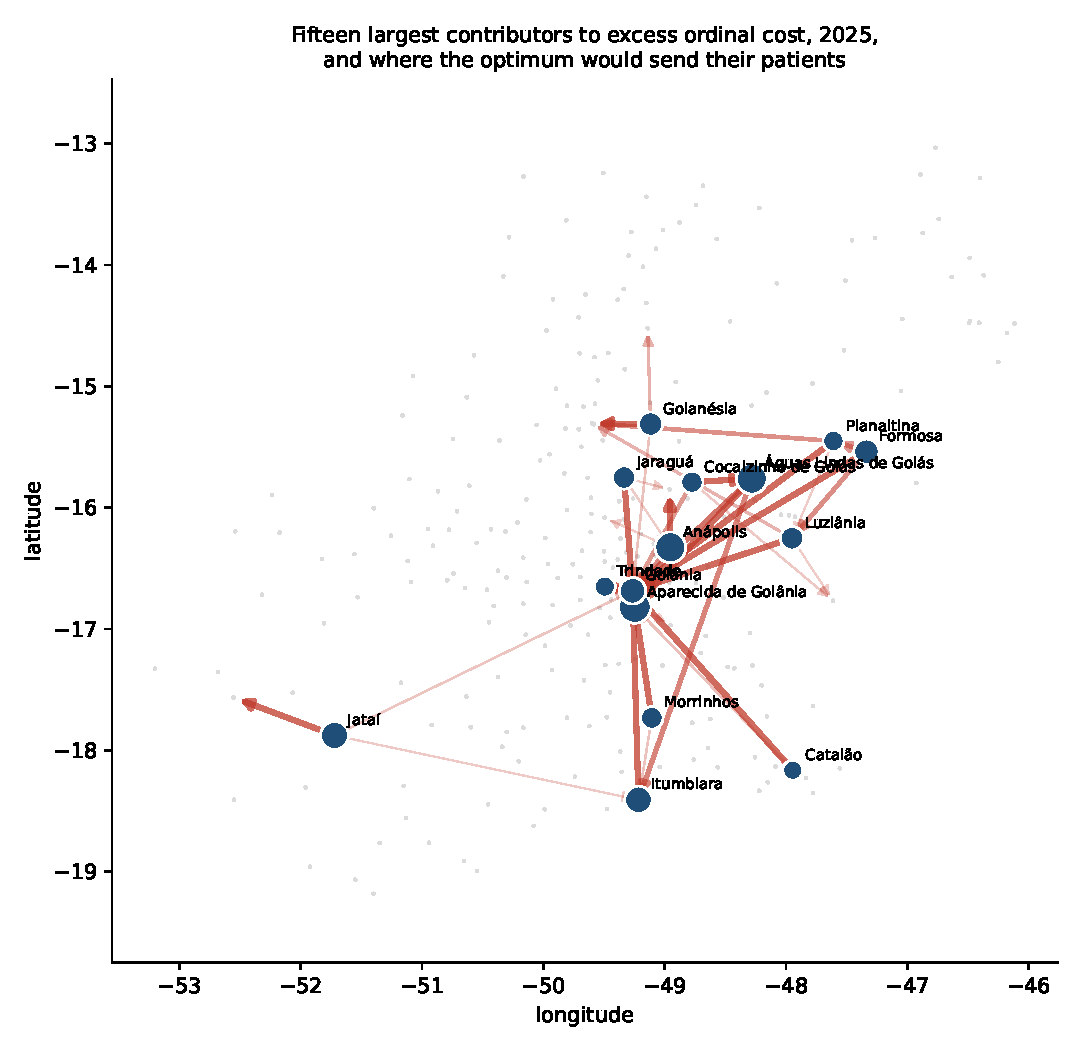
\includegraphics[width=0.82\textwidth]{fig4_worst_served_2025.pdf}
\caption{The fifteen municipalities contributing most to excess ordinal cost in 2025,
sized by that contribution, with arrows to the three municipalities the optimum
sends most of their volume to. Grey points are the remaining municipal seats.
Most arrows are short: the reassignment the model proposes is largely local.}
\label{fig:worst}
\end{figure}

The two diverge afterwards, in a way that illustrates the pattern at the scale
of a single municipality. Valpara\'iso has no facility with elective volume at
any of the three dates; its optimal cost falls from 2.42 to 1.55 and then holds
there, moving only because provision elsewhere moved nearer, and none of its
volume is served at home in any solution. \'Aguas Lindas acquires one facility
in SIH Goi\'as between 2019 and 2023, carrying two facility-procedure pairs, and six pairs by
2025; the optimum keeps none of its volume locally in 2019, 32 per cent in 2023
and 70 per cent in 2025, and its optimal cost falls from 2.54 to 1.68 to 0.91. The arrival of one facility carrying two facility-procedure pairs moves that municipality most of the way to the frontier in the model.

The ranking is positively correlated across the panel. The Spearman rank correlation of excess ordinal cost across the 246 municipalities is 0.737 between 2019 and 2023, 0.685
between 2023 and 2025, and 0.675 between the endpoints; ten, ten and eight of
the fifteen largest contributors carry over between the same pairs of years.
Aparecida de Goi\^ania is among the three largest at every date and An\'apolis
among the four, with the same structure throughout: observed cost well above an
optimum attainable within the patient's own municipality. The distance from the program's optimum recurs in these municipalities across the years examined; whether it reflects misallocation, patient choice, surgeon availability or regulation is not determined here. These municipal figures are computed at a single optimum of the program; a post hoc check in the repository (\texttt{dist/research2/RESULTS.md}, Addendum~3), which did not examine municipalities, finds that quantities below the state level (tested at the health-region level) are identified only at the exact optimum and not among allocations within 1 per cent of it, so the municipal ranks and shares describe the solution reported rather than every near-optimal allocation.

One large contributor does not persist, and the exception is instructive. Rio
Verde ranks first in both 2019 and 2023, at 69.8 and 107.6 units, and last of 246
in 2025 at $-81.9$. Its residents' observed mean cost fell from 0.75 to 0.40 while
their volume rose from 197 to 559 cases per month, and the peak-volume cap summed
over facilities in Rio Verde rose from 223 to 477 cases per month across the same
interval. The excess turns negative because the caps now bind there: the optimum can keep
only 70 per cent of Rio Verde's volume in the municipality, against 96 per cent
in 2019, while observed practice keeps more, so the optimum's mean cost of 0.54
sits above the observed 0.40. This is a property of the
cap rather than evidence of over-performance. A facility may exceed its
three-month rolling mean in an individual month, and where it does, the observed
allocation is locally cheaper than any allocation the model is permitted to
choose. The largest single
distance from the optimum of the first two years closed, in the direction of the
model's ranking, with capability arriving where the patients already were. We do
not claim the model caused this; the quantity it ranks is one that
moves.

\subsection{Uncertainty and the equity margin}
\label{sec:uncertainty}

Every figure above is a point estimate on a single realised panel. We resample
facility-months, re-estimate $\lambda_{jp}$ and the caps on the resampled panel,
and re-solve at the 1$\times$ cap. Two procedures run on the same scheme and
should not be confused: a marginal bootstrap of 300 draws per year, reported
first, and the paired bootstrap of 340 replicates reported below, in which one
weight vector is applied to all three years at once. The scheme is a multiplier
bootstrap: $\kappa$ is a maximum over rolling windows, so any resample that
zeroes facility-months deflates it mechanically, and Dirichlet weights keep every
facility-month present while perturbing its magnitude. The scheme resamples demand, caps, stay
lengths and the observed baseline; it does not resample the bed-day budgets $B_j$, the facility set
$J$ or the option scope, so the intervals understate uncertainty about those.

The gap has a standard deviation of 1.9 points in 2019, 2.6 in 2023 and 2.1 in
2025, with 95 per cent intervals of $[28.0, 35.7]$, $[28.9, 38.5]$ and
$[29.7, 38.0]$. These are intervals from the marginal bootstrap (300 draws). The paired run of Table~\ref{tab:bootvar} gives slightly different endpoints, and the 2025 point estimate lies below the 2025 percentile interval, so neither is used for inference about the level. The replicates resample facility-months of what is close to a census of the state's authorisations, so the intervals describe sensitivity to the monthly pattern and not sampling from a larger population.

Overlapping marginal intervals are weak evidence about a difference, so we test
the differences directly. Drawing one weight vector per replicate and applying it
to all three panels, indexed on facility and month of year so that a facility's
January slot carries the same weight in every year, gives 340 paired replicates.
The between-year differences are then read off within a replicate. The 2023
figure exceeds the 2019 figure by 1.8 points with a 95 per cent interval of
$[-2.2, +6.0]$; 2025 falls below 2023 by 1.5 points, interval $[-5.0, +4.6]$; and
2025 exceeds 2019 by 0.4 points, interval $[-2.9, +6.3]$. None of the three
differences is distinguishable from zero. This is no detectable change, not evidence of equality: the
95 per cent percentile intervals on the differences from this scheme, whose width depends on the weighting dispersion (below), are 8.2, 9.6 and 9.2 points wide, so changes of several points
between years cannot be excluded, and no trend should be read into the ordering of 28.8, 30.6 and 29.1.

The bootstrap means sit 3 to 5 points above the point estimates, and the 2025 point estimate lies below
its own percentile interval (29.1 against $[29.7, 37.8]$). The cause is not convexity in demand alone.
Table~\ref{tab:bootvar} perturbs only part of the inputs. Resampling demand with $\kappa$ held at its point
value lowers the gap, by 0.9, 2.3 and 2.1 points, which is what convexity of the optimal value in demand
implies. Resampling $\kappa$ with demand held fixed raises it, by 1.4, 2.0 and 3.4 points: $\kappa$ is a
maximum over windows, so reweighting months lifts it, loosening the cap. The two effects do not add (the
full-run shifts are 3.3, 3.7 and 4.8 points), so the upward shift in the paper's bootstrap comes from resampling
$\kappa$. We attempted a
bias-corrected and accelerated interval to remove the objection rather than
explain it, with acceleration from a jackknife over facilities. The jackknife
population is the 189 facilities with in-state elective volume in at least one of
the three years, before the restriction to $J$: 134 in 2019, 136 in 2023 and 152
in 2025, unioned. It does
not work here, and the reason is worth stating. Only 1.5 to 4.4 per cent of
replicates fall below the point estimate, so the bias correction $z_0$ runs
between $-1.7$ and $-2.2$, and the corrected endpoints target quantiles of order
$10^{-8}$ and below. With any feasible number of replicates those endpoints are
the smallest draw rather than an estimate. The failure is diagnostic: the
discrepancy is a systematic shift of the resampling distribution, which resampling a maximum
produces, not the skewness that BCa is built to correct. A subsampling variant (an $m$-out-of-$n$
multiplier bootstrap with $m = n/2$ and $0.7n$) did not help: its intervals cover the point estimate in one
of six cases and its means sit higher still. Two further runs of 100 draws each locate the source. With the weight dispersion halved (coefficient of variation 0.5 instead of 1) the upward shift of
the mean falls to 1.7, 2.0 and 2.7 points, about half, so its size depends on the weighting scheme and is not a property of the data alone; with $\kappa$ and demand both held fixed the mean gap lies 0.5, 0.9 and
0.7 points below the point estimate and the interval covers it. A count-matched (multinomial) variant was not run. That resampling a maximum raises the gap is an empirical result for these data and not a theorem; the convexity argument (the optimal value is convex in demand, so demand perturbation lowers the gap) applies to demand with the observed baseline held fixed, which is the $\kappa$-fixed column of Table~\ref{tab:bootvar}. We therefore report the percentile interval together with the
basic interval and the point estimate computed on the realised panel (Table~\ref{tab:bootvar}), and never the
percentile interval alone. The basic interval lies below the percentile interval,
$[22.4, 29.1]$, $[23.0, 30.9]$ and $[20.5, 28.6]$; in 2025 the point estimate (29.1) lies outside both, a symptom of bootstrapping a statistic built on a maximum at a degenerate optimum, so neither is a valid confidence interval. The BCa endpoints, whose target quantiles cannot be estimated, are $[27.3, 29.3]$, $[28.1, 31.3]$ and $[28.2, 28.7]$ against the point estimates 28.8, 30.6 and 29.1, and are not used. We make no interval statement about the level beyond the construction ranges of Table~\ref{tab:measure}.

\begin{table}[t]
\centering
\caption{The bootstrap gap with all inputs, only $\kappa$, or only demand resampled (340 paired draws; per cent). Mean and 95 per cent percentile interval; shift is the mean minus the point estimate in points; ``basic'' is the reverse-percentile interval of the full run, $[2\hat\theta - q_{97.5}, 2\hat\theta - q_{2.5}]$. Stay-length shrinkage over all elective records, as in the stored model; the earlier shrinkage over model facilities only gives the same figures to one decimal. The $\kappa$-fixed and demand-fixed runs leave 0.3 to 0.5 per cent and up to 0.03 per cent of demand unmet, so they are diagnostics, not a decomposition.}
\label{tab:bootvar}
\begin{tabular}{lrrrrr}
\toprule
Year & Point & Full: mean [interval] & $\kappa$ fixed: mean (shift) & Demand fixed: mean (shift) & Full: basic \\
\midrule
2019 & 28.8 & 32.1 [28.5, 35.1] & 27.9 ($-0.9$) & 30.2 ($+1.4$) & [22.4, 29.1] \\
2023 & 30.6 & 34.3 [30.3, 38.1] & 28.3 ($-2.3$) & 32.6 ($+2.0$) & [23.0, 30.9] \\
2025 & 29.1 & 34.0 [29.7, 37.8] & 27.0 ($-2.1$) & 32.5 ($+3.4$) & [20.5, 28.6] \\
\bottomrule
\end{tabular}
\end{table}


\paragraph{The equity margin.} The objective minimises the state-wide mean, which
is not what a secretariat is accountable for. Adding a cap $\tau$ on each
municipality's own mean cost and sweeping it traces the trade. Unmet demand is
forced to zero throughout, because otherwise a tighter $\tau$ is met by dropping
the expensive cells and the served-only mean falls as the constraint tightens,
which is the artifact of Section~\ref{sec:formulation} rather than a frontier.

On 2025 the trade is not a trade. Requiring every municipality to average no more
than 2.5 index units raises the mean cost index by 0.25 per cent, from 0.6419 to 0.6435. Below that the program is infeasible at full service, and
it is infeasible at any aggregate cost, not merely an expensive one. Every
value of the ceiling tried below 2.5 (2.25, 2.0 and lower) is infeasible at full service. We did not
test whether that is because the nearer options are at their caps or because the options are too
far away, so no explanation is offered.

The equity constraint is therefore close to free until it becomes unattainable. Within this program there is no allocation of the existing capability that serves the worst-off municipalities well. We did not test why a ceiling below 2.5 is infeasible and draw no inference from it about instruments.




\section*{Conclusion}
Elective surgery in Goi\'as roughly doubled between 2019 and 2025, and most of the facility-procedure pairs present in 2023 and absent in 2019 were already active in the record in 2020 to 2022. The constructed bed-day budget was slack in aggregate; one, three and six facilities used more than 95 per cent of it. A transparent assignment benchmark shows no detectable change in the gap, but its level depends on how the cap, the cost, the zones and the bed budget are built, and the tests we ran on the cap are low-power or
not identified. The paper therefore claims a description and a benchmark with stated limits, not a cause or a policy lever. The most useful next steps are data that
the SIH files lack: the hospital contract targets, Goi\'as residents treated in the Federal District, and waiting times.

\section*{Declarations}
\paragraph{Code and data availability.} Code, automated checks and a record of corrections: \url{https://github.com/l0mb3ll0/sus-goias-elective-surgery}. The source data are public: SIH/SUS and CNES files from DATASUS (Minist\'erio da Sa\'ude) and municipality and region codes from IBGE; \texttt{data/README.md} names each source. Files containing professional identifiers are not distributed. The reproduction script rebuilds the model-based stored numbers from a clean checkout; the review-pass results (optimal-face searches, null simulations, bootstrap variants, sensitivity rows) come from separate scripts in \texttt{dist/review} that it does not run. The checks re-run the same code; they are reproducibility checks, not independent verification of correctness.
\paragraph{Funding.} None.
\paragraph{Competing interests.} None.
\paragraph{Acknowledgments.} AI-assisted tools were used to support data processing and code development. The author designed the study, verified all results and takes full responsibility for the content.
\paragraph{Ethics.} This study uses only publicly available, de-identified administrative data published by the Brazilian Ministry of Health (DATASUS SIH/SUS and CNES). Professional-level files were used only to compute facility-level counts of registered surgeons (Section~\ref{sec:capnull}); no individual-level data are reported.


\appendix
\section{Exploratory extension: opening new facility-procedure pairs}
\label{app:explore}

This appendix is exploratory. It rests on an assumed capability for new pairs, was not validated by choosing pairs on one year and evaluating them on a later one, and uses demand that omits Goi\'as residents treated in the Federal District. It supports no recommendation.

\subsection{Was capability placed where the model priced it?}
\label{sec:placement}

Because equation~\eqref{eq:cap} is a constraint rather than a bound, its dual is
available at no extra cost, and it has a direct reading: the shadow price on
$\kappa_{jp}$ is the marginal reduction in the program's objective, in index units per
month (at the 2023 optimum all demand is assigned and relaxing a cap cannot create unmet demand, so the change falls on the cost index alone), from one additional unit of permitted volume under the historical peak-cap rule at facility $j$ for
procedure $p$. In the 2023 solution 143 pairs carry a positive dual, 95 of them
non-floored, and the largest reach the ceiling of 3 index units per case,
the value of treating locally a patient who otherwise leaves their intermediate
region entirely. This is the priced object of the exploratory extension in Appendix~\ref{app:explore}, and it
requires no assumption about what opening a pair would cost.

Three properties of this dual vector should be stated before it is used. The
population is the pairs in scope, 517 of the 637 in 2023 being non-floored, which
is a larger set than the 490 used and non-floored pairs that Section~\ref{sec:formulation}
uses as the denominator for binding shares: a pair carrying no flow is still a
candidate for capability. The dual vector is degenerate. Of the 249 non-floored
pairs at their cap in 2023, only 95 carry a positive shadow price and 154 carry
zero, which is ordinary for a transport-like program with many alternative optima
and is not an error. But it means the dual vector is not unique, so any ranking
built on it is partly a property of the solver rather than of the system. We test
this directly by re-solving with the objective perturbed by uniform noise of
$10^{-4}$, twenty times. The Spearman rank correlation of the dual vector against
the unperturbed solution averages 0.73 and never falls below 0.72, and 78 per cent
of the top fifty pairs are retained on average, never fewer than 74. The ranking
is therefore informative but not sharp, and Section~\ref{sec:extension} treats a
dual-ranked list as a screen to be verified rather than as an answer.

It also supports a test. If the model has normative content, capability added
between 2023 and 2025 should have appeared disproportionately where the 2023
solution priced it highly. We rank pairs by dual times a fixed increment of five
cases per month and ask what share of subsequent capability growth landed in the
top decile, against a null in which the top decile is drawn at random with
probability proportional to facility size, so that a result cannot be produced by
large facilities simply growing more.

The literal form of this test is not identified: a pair absent from the 2023
option set has no 2023 dual, so pairs absent in 2019 cannot be scored on the
ranking they would be tested against. We run it on the two margins that are
identified. On the pair margin, across those 517 non-floored 2023 pairs, 17.1 per
cent of the 1{,}875 cases per month of subsequent growth in $\kappa_{jp}$ landed
in the top-valued decile, against a null mean of 14.1 per cent and a null 95th
percentile of 22.4 ($p = 0.26$). On the facility margin, 13.7 per cent of the 131
pairs new in 2025 appeared at the top decile of facilities by summed 2023 value,
against a null mean of 9.3 per cent and a 95th percentile of 14.5 ($p = 0.10$).

Both point the right way and neither is distinguishable from size-weighted random
placement. Whether that is informative depends on what the test could have
detected, so we report it. On the pair margin the null's 95th percentile is 22.4
per cent, and allowing for the spread of the alternative the test rejects a true
concentration of 26.5 per cent or more with 80 per cent power, against a null mean
of 14.1: it resolves a lift of about 1.9 times. On the facility margin the
corresponding figures are 14.5 and 17.0 per cent against a null mean of 9.3, again
a lift of about 1.8 times. A test that would have found capability going to the
priced pairs at roughly twice the rate chance predicts did not find it. The test's minimum detectable lift is about 1.8 to 1.9 times chance, so it does not exclude
a tilt of up to roughly that size, and pairs that are new in the later year (entrants) are excluded from it
by construction.

The test does not detect concentration of new capability at the priced pairs. Rio Verde, where local capability
more than doubled and the largest single distance from the optimum in the panel closed, is a single visible case, not a pattern the test detects.

The test finds no detectable concentration, and it could not have detected lifts below about 1.9 times chance, so we draw no conclusion about whether capability placement is aimed at the priced pairs. A ranking of the kind above
is therefore a model output, not a description of SES-GO practice or a recommendation, and Section~\ref{sec:extension} treats it accordingly.
Two cautions carry into any such use. The floor of $0.5$ generates high duals at
pairs whose cap is a construct rather than a measurement, so floored pairs must be
excluded before ranking. And where the facility total also binds, which
Section~\ref{sec:formulation} shows is the majority case, a pair's dual overstates what
relaxing that pair alone would buy.


\subsection{What a budget of new capability would buy}
\label{sec:ksweep}

Section~\ref{sec:placement} finds no detectable concentration of new capability at the priced pairs. A separate exploratory question is which pairs the program would open, and it can be posed without the pair-opening cost the data does not contain. Fix a budget of
$k$ new facility-procedure pairs, let the program choose which to open, and sweep
$k$. No price enters anywhere.

Formally, a binary $y_{jp}$ is added for each candidate pair, a pair at a facility
in $J$ for a procedure that facility does not currently perform, with
$\sum_{jp} y_{jp} \leq k$ and a cap of $y_{jp}\hat{\kappa}_{jp}$ in place of
$\kappa_{jp}$. Everything else is the program of equation~\eqref{eq:cap}
unchanged. In particular the facility total and the bed-day row still bind on
opened pairs: a facility that is already at its total cap may re-mix its caseload
but may not do more of it. That is a deliberate reading, and
Section~\ref{sec:formulation} shows it is the majority case.

Three quantities have to be assumed rather than measured, and each is stated
rather than tuned. A newly opened pair receives capability $\hat{\kappa}_{jp}$
equal to the median $\kappa_{jp}$ for that procedure among facilities in the same
bed-size tercile, swept at $0.5\times$, $1\times$ and $2\times$ as a ladder in the
manner of Table~\ref{tab:modelrobust}. A new pair has no facility-specific length
of stay and receives the procedure-level mean. And a candidate pair is linked only
to municipalities within cost 1, its facility's own municipality or immediate
region, because opening capability to serve patients two regions away is not the
policy this represents. Of 1{,}471 candidates, the 400 with the largest values in
the linear relaxation are carried into the integer program. The optimality gaps
reported below are therefore gaps on that restricted problem, and every value in
Table~\ref{tab:ksweep} is a value for that restricted problem under the three assumptions above. We
do not call the gains conservative: the capability assumed for a new pair, the candidate arcs, the stay length and the omitted
Entorno demand could each move them in either direction, and choosing pairs on one year and evaluating them on a later one
was not done.\footnote{The screen does not bind at these budgets. Across all
eleven budgets and all three $\hat{\kappa}$ levels, 81 distinct candidates are
ever selected, 55 of them at the central level, leaving 319 of the 400 screened
candidates never chosen. A screen that is never exhausted cannot be excluding a
better solution at $k \leq 50$.}

\begin{table}[t]
\centering
\caption{Reduction in optimal mean travel cost from opening $k$ new
facility-procedure pairs, 2025, as a percentage of the $k=0$ optimum of 0.642.
Columns are the assumed capability of an opened pair, as a multiple of the
tercile median. Every cell solved to a relative MIP gap below $10^{-3}$.}
\label{tab:ksweep}
\begin{tabular}{lrrr}
\toprule
& \multicolumn{3}{c}{$\hat{\kappa}$ multiplier} \\
\cmidrule(lr){2-4}
Budget $k$ & $0.5\times$ & $1\times$ & $2\times$ \\
\midrule
1  & 0.60\%  & 0.72\%  & 1.29\%  \\
2  & 1.17\%  & 1.45\%  & 2.36\%  \\
3  & 1.58\%  & 2.13\%  & 3.34\%  \\
5  & 2.35\%  & 3.40\%  & 4.93\%  \\
8  & 3.37\%  & 5.06\%  & 6.95\%  \\
12 & 4.60\%  & 6.84\%  & 9.05\%  \\
16 & 5.64\%  & 8.33\%  & 10.54\% \\
20 & 6.61\%  & 9.48\%  & 11.77\% \\
30 & 8.49\%  & 11.55\% & 13.91\% \\
40 & 9.85\%  & 13.12\% & 15.46\% \\
50 & 10.90\% & 14.26\% & 16.54\% \\
\bottomrule
\end{tabular}
\end{table}

Table~\ref{tab:ksweep} reports the frontier. The gains are large and concave.
Twenty new pairs, at the central assumption, cut the optimal mean cost index by 9.5 per cent; fifty cut it by 14.3. Put against the observed allocation, the attainable
frontier moves from 29.1 per cent below observed with the capability that exists
to 35.8 per cent at $k=20$ and 39.2 at $k=50$. In the model, twenty opened pairs widen the benchmark gap from 29.1 to 35.8 per cent of the observed index, about a quarter more than reallocation alone. These are values of an exploratory program under assumed capability for new pairs, with demand that omits Entorno residents; they are not a recommendation.

\paragraph{The choice is only partly identified.} The frontier is robust to
$\hat{\kappa}$ in shape but the identity of the chosen pairs is not, and that is a
finding rather than a nuisance. At $k=1$ the three levels choose three different
pairs, with no overlap at all; at $k=3$ the pairwise Jaccard overlaps are 0.20,
0.50 and 0.00. Which single capability is most valuable depends entirely on how
much capability one assumes it comes with, and the data does not identify that.
Agreement improves with the budget: at $k=20$ the pairwise overlaps are 0.60,
0.67 and 0.43, and twelve of the twenty pairs are chosen at all three levels.
The defensible object is therefore a set of roughly a dozen, not a ranked
shortlist of three, and any recommendation phrased as ``open this pair first''
would be reading the assumption rather than the data.

Where that core sits is itself informative. At $k=20$ under the central
assumption the openings concentrate in Luzi\^ania and Rio Verde, four each, then
Ceres and Aparecida de Goi\^ania with two, and by subgroup they are: nine in oncological surgery (0416), four in circulatory-system surgery (0406), four in musculoskeletal surgery (0408) and three in other surgeries (0415). Of the twelve pairs chosen at all three levels, six are in oncological surgery and three each in circulatory-system and musculoskeletal surgery. Under the central assumed-capability scenario and this candidate set, the exploratory model selects pairs closer to recorded demand; this is a scenario result, not evidence of which pairs should be opened. The same direction appears in Section~\ref{sec:flows}, from the flow matrix, and Section~\ref{sec:capbind}, from the binding pattern.

\paragraph{Solve times.} The three sweeps took 733, 878 and 976 seconds in total
across eleven budgets each, on a single core through HiGHS. Every cell reported
closed to a relative gap below $10^{-3}$ within a 150-second limit. An earlier
pass at a 45-second limit did not: at $\hat{\kappa} = 0.5\times$ and $k = 50$ the
solver returned a feasible point worse than doing nothing, with a relative gap of
1. That is recorded here rather than dropped, because a budget of 50 cannot be
worse than a budget of 40 and an incumbent that says otherwise is a solver
artifact, not a result.


\subsection{Validation and extension}
\label{sec:extension}

The endogenous-opening extension, deferred in earlier drafts, is no longer
outstanding.
Section~\ref{sec:ksweep} implements it under a budget rather than a price, which
is what makes it feasible: the pair-opening cost the data does not contain never
has to be supplied. What that section cannot do is compare the chosen pairs with
those that actually appeared on equal terms, because $\hat{\kappa}$ is assumed
and the choice at small budgets turns out to depend on it. A cost-based variant
would still be worth having if pair-level capital and staffing costs could be
obtained from SES-GO, which we have not attempted.

Two questions do remain, and neither is answerable with the data in hand.

First, is the 2025 plateau a constraint? State-administered facilities
plateau at approximately 151 elective cases per facility-month in the final regime (April to December 2025; mean over state-administered facility-months with elective volume) while municipal-administered facilities continue to climb, a pattern
consistent with an operating-room session constraint distinct from the bed-day
budget. The 2025 instance is solved above and has the lowest ratio of cap to demand of the three years, but the session constraint is not imposed
separately from the bed-day budget and the two cannot be distinguished on SIH
alone. Testing it requires operating-room session data the billing record does
not contain.

Second, does the objective survive replacement? The travel-penalised formulation
is the defensible choice given that SIH records no queue registration date and
therefore no waiting time. A request for aggregate queue
extracts from the state regulation system is pending. Were it to return, a
weighted-tardiness objective becomes estimable and should be reported alongside.
\section{Timing of the 2022 change and growth across facilities (descriptive)}
\label{app:timing}

These subsections describe when and where elective volume grew in 2022. They do not identify the cause of the growth.

\subsection{The 2022 change occurred in two waves}

The 2022 break date is not stable across specifications, and the instability is
informative rather than a nuisance. On the full sample PELT returns May 2022;
on the reliable subset it returns October 2022; a single-changepoint search
returns September. Running the reliable-subset series at a lower penalty
returns both May and October.

Inspection of the seasonally adjusted series shows why. The ratio is 0.334 in
January and February 2022, then 0.522, 0.493, 0.546, 0.510 and 0.505 from March
to July, then 0.665 in August. A fixed-cardinality search with two breaks over
the window June 2021 to June 2023 returns April 2022 and September 2022, with
segment means of 0.400, 0.469 and 0.633. There are two steps, not one, and
single-changepoint procedures report a date between them.

The two steps involve different sets of facilities. Classifying reliable-subset
hospitals by whether their volume grew by more than 30 per cent across the
first step (August 2021 to February 2022 against March to July 2022) or the
second (March to July 2022 against August 2022 to January 2023) gives nine
facilities that move only in the first, twelve that move only in the second,
six that move in both and twenty-two that move in neither, on the 49 facilities
clearing five elective cases per month in the August 2021 to February 2022 base
window. The correlation between the two growth ratios is $-0.04$ (Pearson),
$-0.22$ in logs and $-0.07$ by rank. Weighted by volume, second-wave movers
contribute 1{,}147 elective cases per month by late 2022 against 461 for
first-wave movers.

Two checks say this is not an artefact. Dropping the low-base rule and using all
61 facilities gives fourteen, thirteen, ten and twenty-two (59 facilities with a defined growth ratio; two are undefined), with correlations of
$+0.03$, $+0.03$ and $-0.01$. And the two ratios share the window March to July
2022, which mechanically depresses their correlation, so we split that window and
recompute with independent denominators: the first step measured to May and the
second from June. Across the full 61 and both subsets the nine resulting
correlations run from $-0.07$ to $+0.13$. The sign is not stable across these
cuts and no weight should be placed on it; what is stable is that all of them sit
near zero, and that facilities moving in both waves stay a clear minority, six of
49 and ten of 59. The movers in the two waves are uncorrelated across facilities.

The case mix, by contrast, moves the same way in both steps. Across four-digit
SIGTAP subgroups the share changes in the first and second steps correlate at
0.86: subgroup 0407 gains 2.75 and then 2.89 percentage points of share, 0415
gains 1.40 and then 1.32, while 0406 and 0416 lose share in both. In SIGTAP these are, respectively, surgery of the digestive system, annexed organs and abdominal wall (0407), whose highest-volume member is laparoscopic cholecystectomy; other surgeries (0415); surgery of the circulatory system (0406), led by bilateral varicose vein repair; and oncological surgery (0416). Geographically, the state's
largest municipality by surgical volume grows by a factor of 1.0 in the first
step and 1.4 in the second, while several interior municipalities grow by
factors between 2.5 and 4.5, at different times. This is measured at
municipality level; the \emph{regi\~ao de sa\'ude}, along which such a reform is
actually rolled out, is not carried in the SIH reduced files.

These patterns are compatible with staged policy implementation, but they do not establish that a policy caused the changes in procedure mix or the timing of facility-level growth.


\subsection{The July 2022 step came from existing facilities}
\label{sec:appb2}

The number of facilities performing elective surgery does not change at the
break. Monthly counts of distinct CNES codes with positive elective volume
range from 94 to 113 across 2022 with no discontinuity in August, against a 26
per cent increase in monthly volume between July and August. Partitioning
facilities into those active in the first half of 2022 and those not, the
July-to-August increase of 1{,}215 elective cases decomposes into 1{,}210 from
facilities already active and 5 from facilities not active in that window.
Facilities with no elective volume in the first half of 2022 remain below
2 per cent of volume through 2022.

Concentration falls. The Herfindahl-Hirschman index of elective volume across
facilities averages 479 over the pre-break window and 398 over the post-break
window; the number of facilities accounting for 90 per cent of volume moves
from the low forties in the first half of 2022 to around fifty in the second.
Volume rose without the distribution across facilities becoming more
concentrated.

The step increase was therefore obtained on the intensive margin: the same
physical facilities produced substantially more elective surgery. Whether they
did so by using existing capacity more fully or by adding staff and equipment
cannot be settled from SIH alone. Cases per surgical bed-month across the break
are reported in Section~\ref{sec:provider}, and show that the additional volume
did not exhaust the constructed bed-day budget: throughput per bed rose in both provider groups without either exhausting it. The corresponding measurement on
staffing has not been made, so activation of latent capacity and silent capacity
expansion cannot be distinguished here.

\paragraph{The longer horizon is different.} The intensive-margin finding is a
statement about the discontinuity, not about the expansion as a whole. Over the
full 2019 to 2023 interval the composition of the increase inverts. Comparing
the set of facility-procedure pairs observed in 2019 with those observed in
2023, both at the four-digit level at which the model of Section~\ref{sec:model}
routes, 284 pairs are present in 2023 and absent in 2019, carrying 21{,}845
elective cases, 27.5 per cent of 2023 volume. A further 192 pairs present in
2019 are absent in 2023, so the pair
count rises from 574 to 666 on gross churn of 476. These counts are over every
facility with elective volume. The option sets of Section~\ref{sec:model}, 563
and 637, are the same quantity restricted to facilities that also have non-zero
net surgical bed capacity, which is why their net change is 74 rather than 92. Of these, 18{,}370 cases are at facilities that report no elective
surgical volume at all in 2019, against 3{,}475 cases from procedures newly
performed at facilities already active in 2019.
A single facility accounts for the largest share: CNES 9680977 billed 3{,}185
AIH in 2019 with zero elective volume and reached 5{,}568 elective cases in
2023, a conversion of an urgent-only unit to elective provision rather than a
new entrant. Of the thirty facilities carrying the 18{,}370 cases, seventeen
appear in the 2019 SIH file with non-elective admissions, several at substantial
volume: CNES 2517949 billed 4{,}262 admissions in 2019, 2534584 2{,}416, 2442728
1{,}741 and 2769603 1{,}231. Absence from the elective data is not absence from
the system. Measured against the elective subset the extensive share is 84.1 per
cent; counting only facilities absent from SIH altogether it is 52.0 per cent.
The second is the
conservative reading and the one we rely on.

\paragraph{Endpoint-year comparisons obscure the timing of recorded activity.}
The comparison above treats a pair as a state, present in a year or absent from
it, and the monthly panel does not support that reading. Of the 284 pairs absent
in 2019, 195 are active in at least one month of 2020, 2021 or 2022, with a
median of five active months and ten cases before 2023 and 13{,}132 cases
between them. They carry 20{,}568 of the 21{,}845 cases, so of the 27.5 per cent
of 2023 volume attributed to pairs absent in 2019, 25.9 points are pairs
with activity in the intervening years, and 1.6 points are pairs
with no recorded activity anywhere in 2019 to 2022. The reverse holds for the
losses: 62 of the 192 pairs absent in 2023 are active again in 2024 or 2025.
The set difference between two endpoint years therefore mixes entry during the
window with intermittent activity; the panel does not observe activity before
2019, so it cannot say which pairs returned after an earlier spell.

This does not disturb the decomposition of Section~\ref{sec:decomp}. A pair dark
across the estimation year has no observable throughput, so its peak-volume cap is
undefined and the optimum cannot route to it whatever it did in an earlier year;
and configuration C is solved on the 2019 option set including the pairs that
later disappeared. The improvement from C to D is unaffected. What changes is the
description of what appeared, not whether it appeared.
Section~\ref{sec:decomp} shows that under the model's rules the 2023 volume is fully assignable only with the 2023 pairs and caps; it makes no attribution between the two.


\subsection{Growth was highly unequal across facilities}

Figures~\ref{fig:hist} and \ref{fig:scatter} report the distribution of the
facility-level growth ratio, defined as mean monthly elective volume from
August 2022 to June 2023 divided by mean monthly volume from January to July
2022, on the reliable subset.

The median facility grew by 35 per cent. But seventeen of fifty-four
facilities did not grow at all, and ten more than doubled, six of them by a
factor above three, on the 54 facilities clearing five elective cases per month
in the January to July 2022 base window. Dropping that rule and using all 61
moves the median from 1.35 to 1.38 and leaves the shape unchanged below twice,
while the mean rises from 1.9 to 3.9 and the maximum from 15 to 105, which is the
instability the rule exists to prevent. The dispersion is the finding, not the
central tendency, and it is larger without the rule than with it.

\begin{figure}[t]
\centering
\begin{minipage}[t]{0.45\textwidth}
\centering
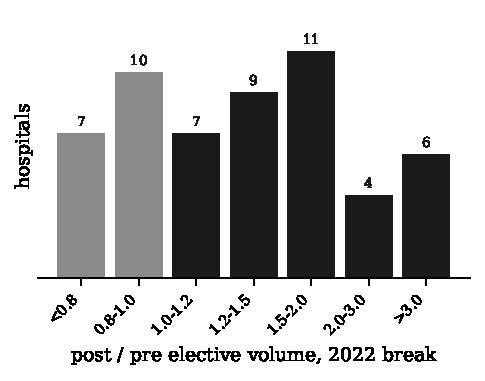
\includegraphics[width=\textwidth]{fig2_growth_histogram.pdf}
\caption{Distribution of facility-level growth ratios across the 2022 break,
reliable subset.}
\label{fig:hist}
\end{minipage}\hfill
\begin{minipage}[t]{0.5\textwidth}
\centering
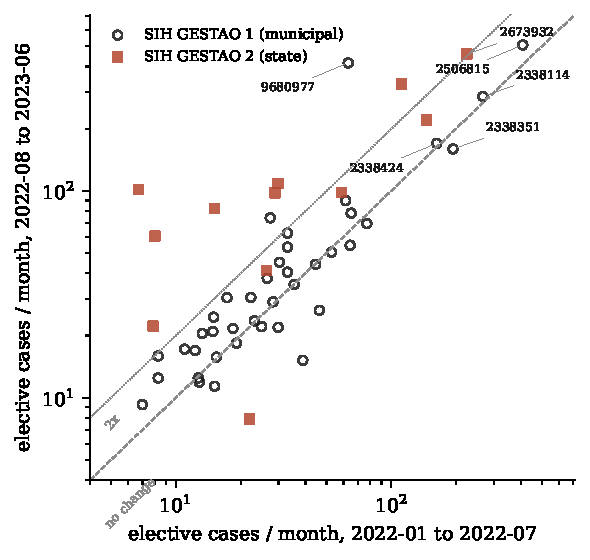
\includegraphics[width=\textwidth]{fig3_pre_post_scatter.pdf}
\caption{Monthly elective volume before and after the break, by facility, log
scale. Points on the dashed line did not change. The largest facilities lie on
or near it.}
\label{fig:scatter}
\end{minipage}
\end{figure}

Figure~\ref{fig:scatter} shows where the dispersion sits. The state's largest
elective surgical facility went from 406 to 538 cases per month, a 32 per cent
increase, and the second largest went from 321 to 263, a decline. Meanwhile a
facility performing 62 elective cases per month before the break performed 366
after it, and one performing 10 performed 95. The facilities that absorbed the
expansion were mid-sized and small units operating far below the volume of the
leaders, and after the expansion they remained below them.

This dispersion is what motivates the model. Before 2022 elective volume was concentrated in a few large facilities, and Section~\ref{sec:capbind} reports that the constructed bed-day budget was slack in aggregate. Facilities that expanded in 2022 were still operating at their new volumes in 2025, and
we do not identify what caused the expansion. The natural question is how far the realised allocation sits from a benchmark assignment.


\subsection{Falsification and robustness}

Table~\ref{tab:falsification} collects the checks that would have overturned the
result and did not.

Urgent surgical admissions move little at the break, either statewide or within
the state-administered group. Statewide urgent volume rises by 6.4 per cent
between the pre- and post-break windows and urgent volume at state-administered
facilities by 7.7 per cent, against a 38 per cent rise in the elective-to-urgent
ratio measured on admission month. Urgent volume did not fall as elective volume rose. No facility
changes its \texttt{GESTAO} code between July and August 2022, so the
concentration of the increase in state-managed units cannot be an artefact of
reclassification. Rebuilding the entire series on admission date rather than
processing month leaves the break in the same month and of the same magnitude:
the pre-window mean is 4{,}013 elective admissions per month at a ratio of
0.471 and the post-window mean is 6{,}108 at a ratio of 0.652. The submission
lag for elective admissions does not rise across the break; measured on the same
windows as the rest of the table it falls, from 0.645 months to 0.629, a change
of two and a half per cent or about half a day. The rise Section~\ref{sec:measconc} reports is between calendar 2021 and calendar 2022, which is a different
comparison and ends before the post-break window opens. Neither direction can
generate a sustained level shift of this size in any case, and the
admission-date reconstruction puts the break in the same month at the same
magnitude.

\begin{table}[t]
\centering
\caption{Falsification checks. Each row reports a quantity that would have
moved if the corresponding alternative explanation were correct.}
\label{tab:falsification}
\small
\begin{tabular}{lrrr}
\toprule
Quantity & Pre & Post & $\Delta\%$ \\
\midrule
Urgent surgical admissions, statewide & 8,554.86 & 9,102.73 & +6.4 \\
Urgent admissions, state-administered units & 3,940.86 & 4,246.09 & +7.7 \\
Hospitals with $>0$ elective cases & 105.00 & 107.36 & +2.3 \\
Concentration (HHI), elective & 479.05 & 398.19 & -16.9 \\
Elective cases, facilities absent pre-break & 0.00 & 8.00 &  \\
Facilities changing SIH management code at the break (of 101) & 0.00 & 0.00 &  \\
Mean submission lag, elective (months) & 0.65 & 0.63 & -2.6 \\
Elective/urgent ratio, by admission month & 0.47 & 0.65 & +38.4 \\
\bottomrule
\end{tabular}

\end{table}



\bibliographystyle{plainnat}
\begin{thebibliography}{99}
\bibitem[Ahmadi-Javid et~al.(2017)]{ahmadijavid2017}
A.~Ahmadi-Javid, P.~Seyedi, and S.~S. Syam.
\newblock A survey of healthcare facility location.
\newblock \emph{Computers \& Operations Research}, 79:223--263, 2017.
\bibitem[Bai and Perron(1998)]{bai1998}
J.~Bai and P.~Perron.
\newblock Estimating and testing linear models with multiple structural changes.
\newblock \emph{Econometrica}, 66(1):47--78, 1998.
\bibitem[Battesini et~al.(2018)]{battesini2018}
M.~Battesini, H.~dos~S. Coelho, and M.~H. De~Seta.
\newblock Uso de programa\c{c}\~ao linear para otimizar o acesso geogr\'afico em redes tem\'aticas de aten\c{c}\~ao \`a sa\'ude.
\newblock \emph{Cadernos de Sa\'ude P\'ublica}, 34(7):e00055017, 2018.
\bibitem[Botega et~al.(2022)]{botega2022}
L.~de~A. Botega, M.~V. Andrade, G.~R. Guedes, and D.~Nogueira.
\newblock Spatial reorganization of the Brazilian Unified National Health System's inpatient care supply.
\newblock \emph{Cadernos de Sa\'ude P\'ublica}, 38(9):e00012422, 2022.
\bibitem[Burdett et~al.(2023)]{burdett2023}
R.~L. Burdett, P.~Corry, P.~Yarlagadda, D.~Cook, S.~Birgan, and S.~M. McPhail.
\newblock A mathematical framework for regional hospital case mix planning and capacity appraisal.
\newblock \emph{Operations Research Perspectives}, 10:100261, 2023.
\bibitem[Dudley et~al.(2000)]{dudley2000}
R.~A. Dudley, K.~L. Johansen, R.~Brand, D.~J. Rennie, and A.~Milstein.
\newblock Selective referral to high-volume hospitals: estimating potentially avoidable deaths.
\newblock \emph{JAMA}, 283:1159--1166, 2000.
\bibitem[Epstein et~al.(2005)]{epstein2005}
A.~J. Epstein, S.~S. Rathore, H.~M. Krumholz, and K.~G.~M. Volpp.
\newblock Volume-based referral for cardiovascular procedures in the United States: a cross-sectional regression analysis.
\newblock \emph{BMC Health Services Research}, 5:42, 2005.
\bibitem[Finlayson et~al.(1999)]{finlayson1999}
S.~R. Finlayson, J.~D. Birkmeyer, A.~N. Tosteson, and R.~F. Nease.
\newblock Patient preferences for location of care: implications for regionalization.
\newblock \emph{Medical Care}, 37:204--209, 1999.
\bibitem[Hamilton(1982)]{hamilton1982}
B.~W. Hamilton.
\newblock Wasteful commuting.
\newblock \emph{Journal of Political Economy}, 90(5):1035--1051, 1982.
\bibitem[Helm and Van Oyen(2014)]{helm2014}
J.~E. Helm and M.~P. Van Oyen.
\newblock Design and optimization methods for elective hospital admissions.
\newblock \emph{Operations Research}, 62(6):1265--1282, 2014.
\bibitem[Killick et~al.(2012)]{killick2012}
R.~Killick, P.~Fearnhead, and I.~A. Eckley.
\newblock Optimal detection of changepoints with a linear computational cost.
\newblock \emph{Journal of the American Statistical Association}, 107(500):1590--1598, 2012.
\bibitem[Luft et~al.(1979)]{luft1979}
H.~S. Luft, J.~P. Bunker, and A.~C. Enthoven.
\newblock Should operations be regionalized? The empirical relation between surgical volume and mortality.
\newblock \emph{New England Journal of Medicine}, 301:1364--1369, 1979.
\bibitem[Luft et~al.(1987)]{luft1987}
H.~S. Luft, S.~S. Hunt, and S.~C. Maerki.
\newblock The volume-outcome relationship: practice-makes-perfect or selective-referral patterns?.
\newblock \emph{Health Services Research}, 22:157--182, 1987.
\bibitem[Marques et~al.(2014)]{marques2014}
I.~Marques, M.~E. Captivo, and M.~V. Pato.
\newblock Scheduling elective surgeries in a Portuguese hospital using a genetic heuristic.
\newblock \emph{Operations Research for Health Care}, 3(2):59--72, 2014.
\bibitem[Meng et~al.(2015)]{meng2015}
F.~Meng, J.~Qi, M.~Zhang, J.~Ang, S.~Chu, and M.~Sim.
\newblock A robust optimization model for managing elective admission in a public hospital.
\newblock \emph{Operations Research}, 63(6):1452--1467, 2015.
\bibitem[Scarpin et~al.(2008)]{scarpin2008}
C.~T. Scarpin, M.~T.~A. Steiner, G.~J.~C. Dias, and P.~J. Steiner Neto.
\newblock Otimiza\c{c}\~ao no servi\c{c}o de sa\'ude no estado do Paran\'a: fluxo de pacientes e novas configura\c{c}\~oes hier\'arquicas.
\newblock \emph{Gest\~ao \& Produ\c{c}\~ao}, 15(2):275--290, 2008.
\bibitem[Scharfe et~al.(2025)]{scharfe2025}
J.~Scharfe, S.~Pfisterer-Heise, A.~Pachanov, C.~M. Kugler, T.~Mathes, Z.~Zhang, J.~Morche, and D.~Pieper.
\newblock The effect of minimum volume standards in hospitals (MIVOS): a systematic review.
\newblock \emph{BMJ Open}, 15(5):e090152, 2025.
\bibitem[Servo et~al.(2021)]{ipea2022}
L.~M.~S. Servo, M.~V. Andrade, and P.~V.~M. Amaral.
\newblock Os caminhos da regionaliza\c{c}\~ao da sa\'ude no Brasil: adequa\c{c}\~ao e acesso geogr\'afico nos anos 2000.
\newblock \emph{Planejamento e Pol\'iticas P\'ublicas}, n.~60 (2021), published online 26 July 2022, 2021.
\bibitem[Small and Song(1992)]{smallsong1992}
K.~A. Small and S.~Song.
\newblock ``Wasteful'' commuting: a resolution.
\newblock \emph{Journal of Political Economy}, 100(4):888--898, 1992.
\bibitem[Vogel et~al.(2022)]{vogel2022}
J.~F.~A. Vogel, M.~Barkhausen, C.~M. Pross, and A.~Geissler.
\newblock Defining minimum volume thresholds to increase quality of care: a new patient-oriented approach using mixed integer programming.
\newblock \emph{European Journal of Health Economics}, 23(7):1085--1104, 2022.
\bibitem[White(1988)]{white1988}
M.~J. White.
\newblock Urban commuting journeys are not ``wasteful''.
\newblock \emph{Journal of Political Economy}, 96(5):1097--1110, 1988.
\bibitem[da Silva et~al.(2010)]{silva2010}
M.~E.~M. da Silva, E.~R. Santos, and D.~Borenstein.
\newblock Implementing regulation policy in Brazilian health care regulation centers.
\newblock \emph{Medical Decision Making}, 30(3):366--379, 2010.
\end{thebibliography}

\end{document}
